\section{演習15}
\subsection{実行プログラム}
実行プログラムをソースコード\ref{s15}に示す。

\begin{lstlisting}[caption=演習15のプログラム,label=s15]
#include <stdio.h>
#include <process.h> /*exit関数の定義*/
#include <dos.h>
#include "v25.h"
#include "ms.h"
  
#define DMAX 10000
#define INTERVAL 100
#define DISTANCE 3000
  
int main(){
    int i, n=0;
    int kp = 3, ki_inv = 10000;
  
    int vref[11] = {1000, 2000, 3000, 4000, 5000, 6000,
                    5000, 4000, 3000, 2000, 1000};
    long time[11] = {200, 200, 200, 200, 200, 1040,
                    200, 200, 200, 200, 200};
    long j=0, cl, cl0, cr, cr0, ct, ct0, ctm, l[DMAX], r[DMAX], t[DMAX];
    FILE *fp;
  
    ms_init();
    ms_motor_on();
    ms_set_gain(kp, ki_inv);
    ms_read_c(&cl0, &cr0, &ct0);
    ctm = ct0;
    for(i=0; i<11; i++){
        ms_set_v(vref[i], vref[i]);
        do{
            ms_read_c(&cl, &cr, &ct);
            n = j/INTERVAL;
            l[n] = cl;
            r[n] = cr;
            t[n] = ct;
            j++;
        }while(time[i]>ct-ctm);
        ctm = ct;
    }
    ms_motor_off();
 
    if((fp = fopen("data.dat", "wt")) == NULL){
        printf("Can't Open File!!\n");
        exit(1);
    }

    for(i=0; i<=n; i++){
        fprintf(fp, "%12.6lf %12.6lf %5ld\n",
        DISTANCE-15*2*3.14159*(l[i]-cl0)/(19.225*400),
        DISTANCE-15*2*3.14159*(r[i]-cr0)/(19.225*400),
        t[i]-ct0);
    }
    fclose(fp);
    ms_beep(440,500);
    return 0;
}
\end{lstlisting}

\subsection{実行結果}
演習14と同様に
モータの応答(回転速度と目標位置までの距離)を
負荷無し、有りの場合分けをしてデータファイルに保存する。
負荷無し、有りの場合を図\ref{fuka_15}、\ref{non_15}に示す。
負荷有りの場合、ロボットは前進しない。
負荷無しの場合、ロボットは目標位置に近づくことが分かる。

\begin{figure}
  \begin{center}
    \subfigure[負荷有り]{
    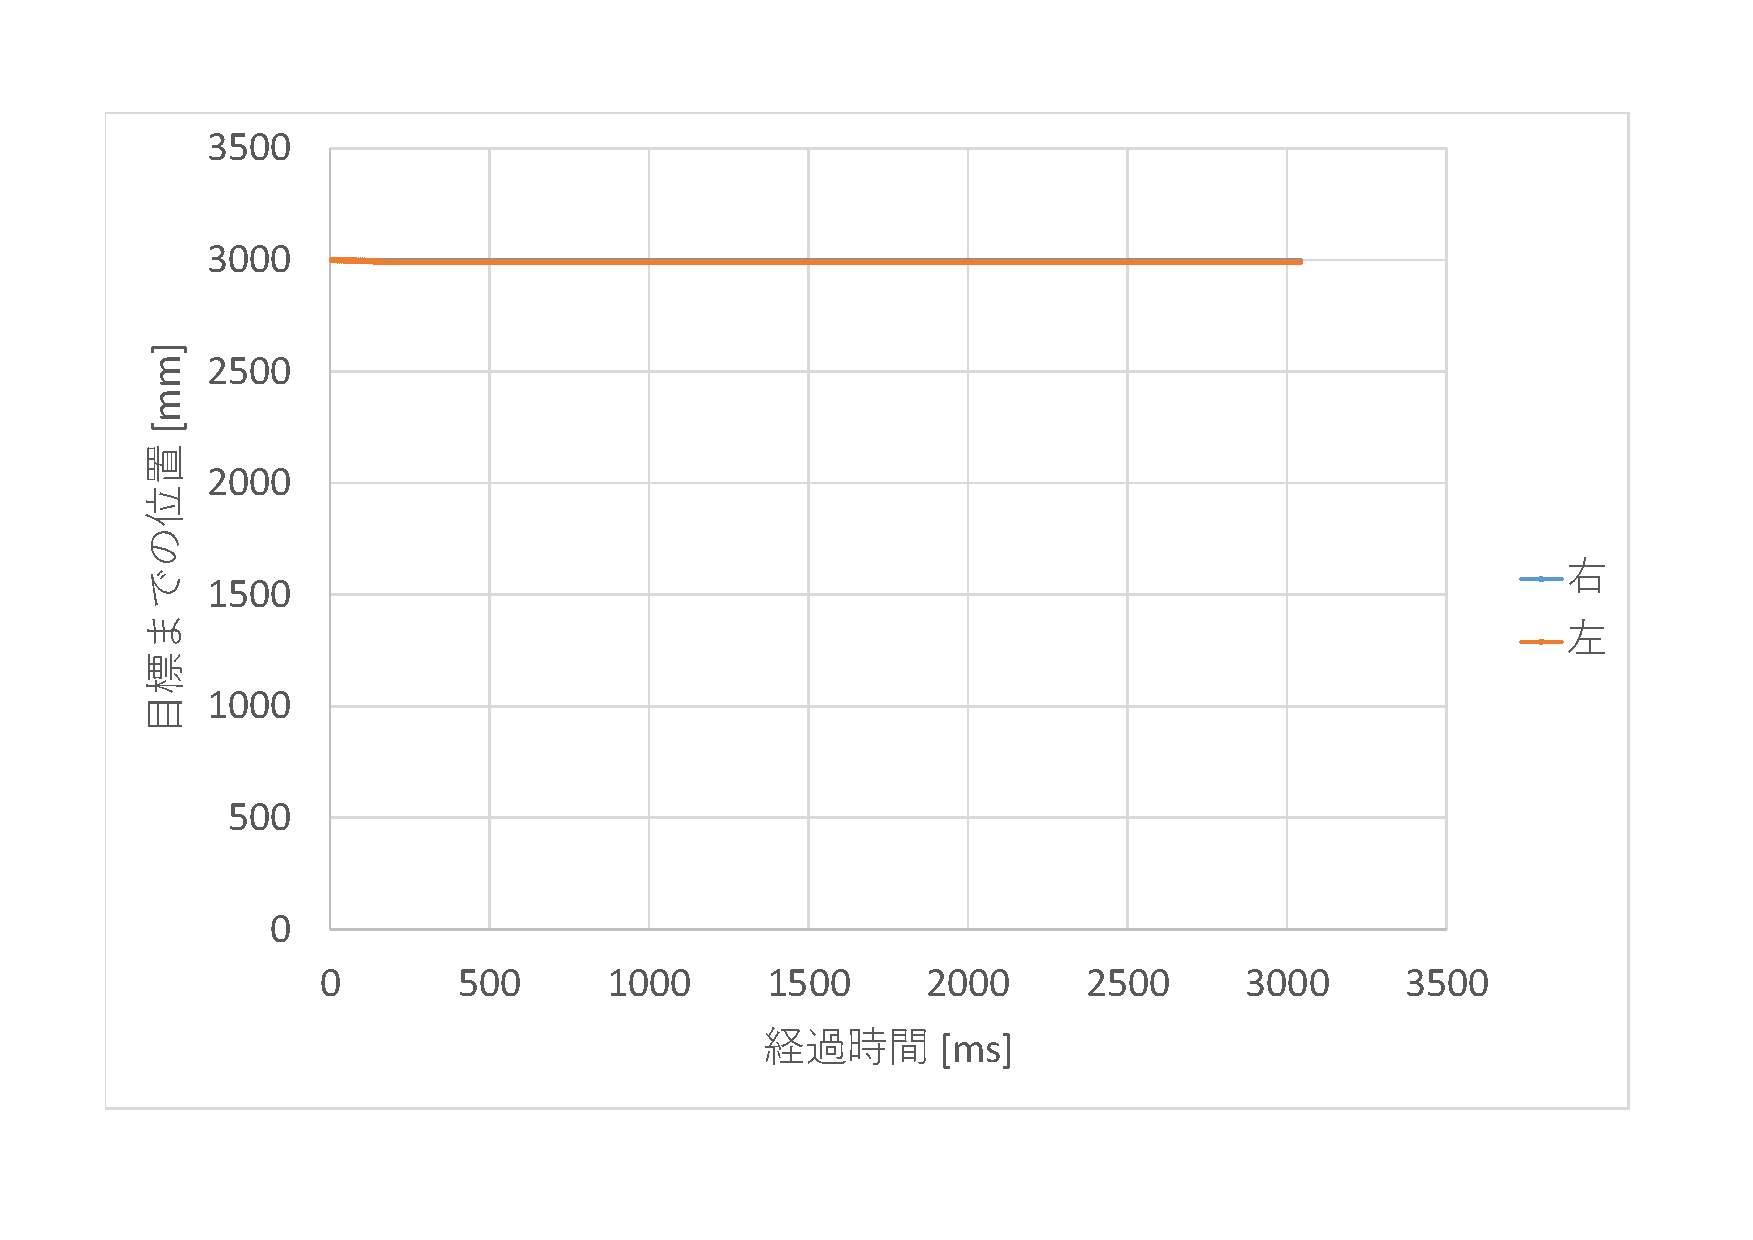
\includegraphics[width=\linewidth]{img/15/15_fuka.pdf}
    \label{fuka_15}
    }
    \subfigure[負荷無し]{
    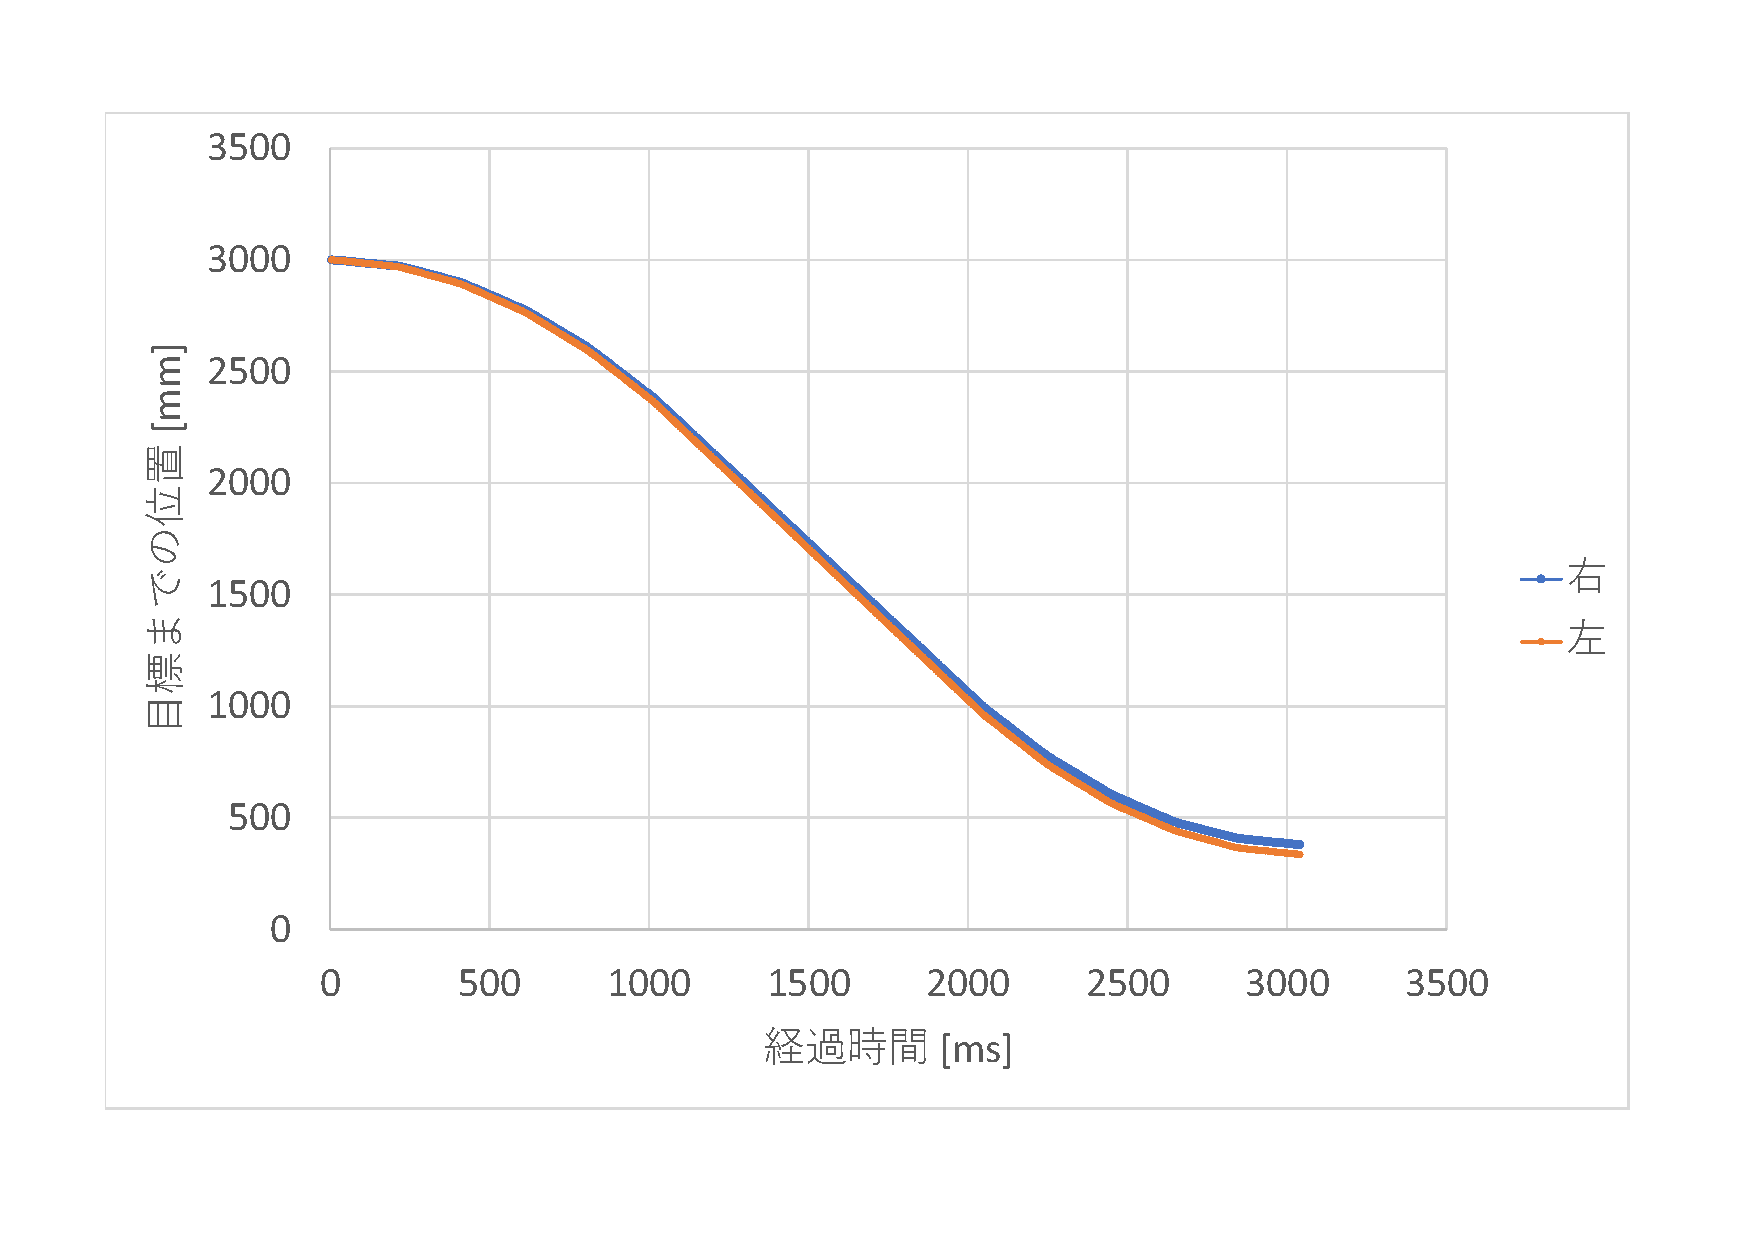
\includegraphics[width=\linewidth]{img/15/15_non.pdf}
    \label{non_15}
    }
  \caption{モータの応答}
  \end{center}
\end{figure}


\section{演習16}
\subsection{実行プログラム}
実行プログラムをソースコード\ref{s16}に示す。
\begin{lstlisting}[caption=演習16のプログラム,label=s16]
#include <stdio.h>
#include <process.h>    /*exit関数の定義*/
#include <dos.h>        /*pokeb関数の定義*/
#include "v25.h"        /*V25固有値の定義*/
#include "ms.h"         /*ms関数の定義*/
   
#define DMAX 10000      /*保存データ数の最大値*/
#define INTERVAL 100    /*保存データの間隔*/
#define INTERVAL2 5     /*保存データの間隔*/
#define DISTANCE 3000   /*ロボットの移動距離*/
#define C_DISTANCE ((DISTANCE*400.*19.225)/(15.*2.*3.14159))
                          /*ロボットの移動距離(カウンタ換算)*/
#define THRESH 100      /*閾値*/
   
int main()
{
    int i, n = 0, n2 = 0, k = 5;
    int kp = 6, ki_inv = 10000;     /*FBゲイン*/
    /*速度パターン*/
    int vref[6] = {1000, 2000, 3000, 4000, 5000, 6000};
    long time[5] = {200, 200, 200, 200, 200};
    long j = 0, cl, cl0, cr, cr0, ct, ct0, ctm, el, er, vl, vr, l[DMAX], r[DMAX], t[DMAX];
    FILE *fp;
  
    ms_init();                          /*初期化*/
    ms_motor_on();                      /*モータ回路ON*/
    ms_set_gain( kp, ki_inv );          /*FBゲインの設定*/
    ms_read_c( &cl0, &cr0, &ct0 );      /*カウンタ値の初期値の取得*/
    ctm=ct0;
    for( i = 0; i < 5; i++)
    {
        ms_set_v( vref[i], vref[i] );   /*速度の設定*/
        do
        {
            ms_read_c( &cl, &cr, &ct ); /*カウンタ値の読み込み*/
            n = j/INTERVAL;
            l[n] = cl;
            r[n] = cr;
            t[n] = ct;
            j++;
        } while ( time[i] > ct-ctm );   /*時間間隔のチェック*/
        ctm = ct;
    }
    j = 0;
    do
    {
        el = C_DISTANCE - cl;           /*目標値との偏差を算出*/
        er = C_DISTANCE - cr;           
        vl = k * el;                    /*速度の計算*/
        vr = k * er;
        if ( vl > vref[5] )             /*最高速度の設定*/
        {
          vl = vref[5];
        }
        if ( vr > vref[5] )
        {
          vr = vref[5];
        }
        ms_set_v( vl, vr );             /*速度の設定*/
        ms_read_c( &cl, &cr, &ct );     /*カウンタ値の読み込み*/
        n2 = j/INTERVAL2 + n + 1;
        l[n2] = cl;
        r[n2] = cr;
        t[n2] = ct;
        j++; 
    } while ( n2<DMAX && el>THRESH && er>THRESH );  /*終了条件のチェック*/
        
    ms_motor_off();                     /*モータ回路OFF*/
    /*保存ファイルのオープン*/
    if ((fp = fopen("data.dat","wt")) == NULL)
    {
      printf("Can't open file.\n");
      exit(1);
    }
    /*ファイルの保存*/
    for ( i = 0; i < n2; i++)
    {
      fprintf(fp,"%12.6lf %12.6lf %5ld\n",DISTANCE-15*2*3.14159*(l[i]-cl0)/(19.225*400),DISTANCE-15*2*3.14159*(r[i]-cr0)/(19.225*400),t[i]-ct0);
    }
    fclose(fp);                     /*ファイルのクローズ*/
    return 0;
}
\end{lstlisting}

\subsection{実行結果}
負荷有りの場合、目標位置までの距離の変化率が左右のモータで均等でない。
ロボットの重心が、左右で均等でなかったためであると考えられる。
負荷無しの場合、目標位置までの距離が単調的に減少し、目標位置に近づくことが分かる。
\begin{figure}[H]
  \begin{center}
    \subfigure[負荷有り]{
    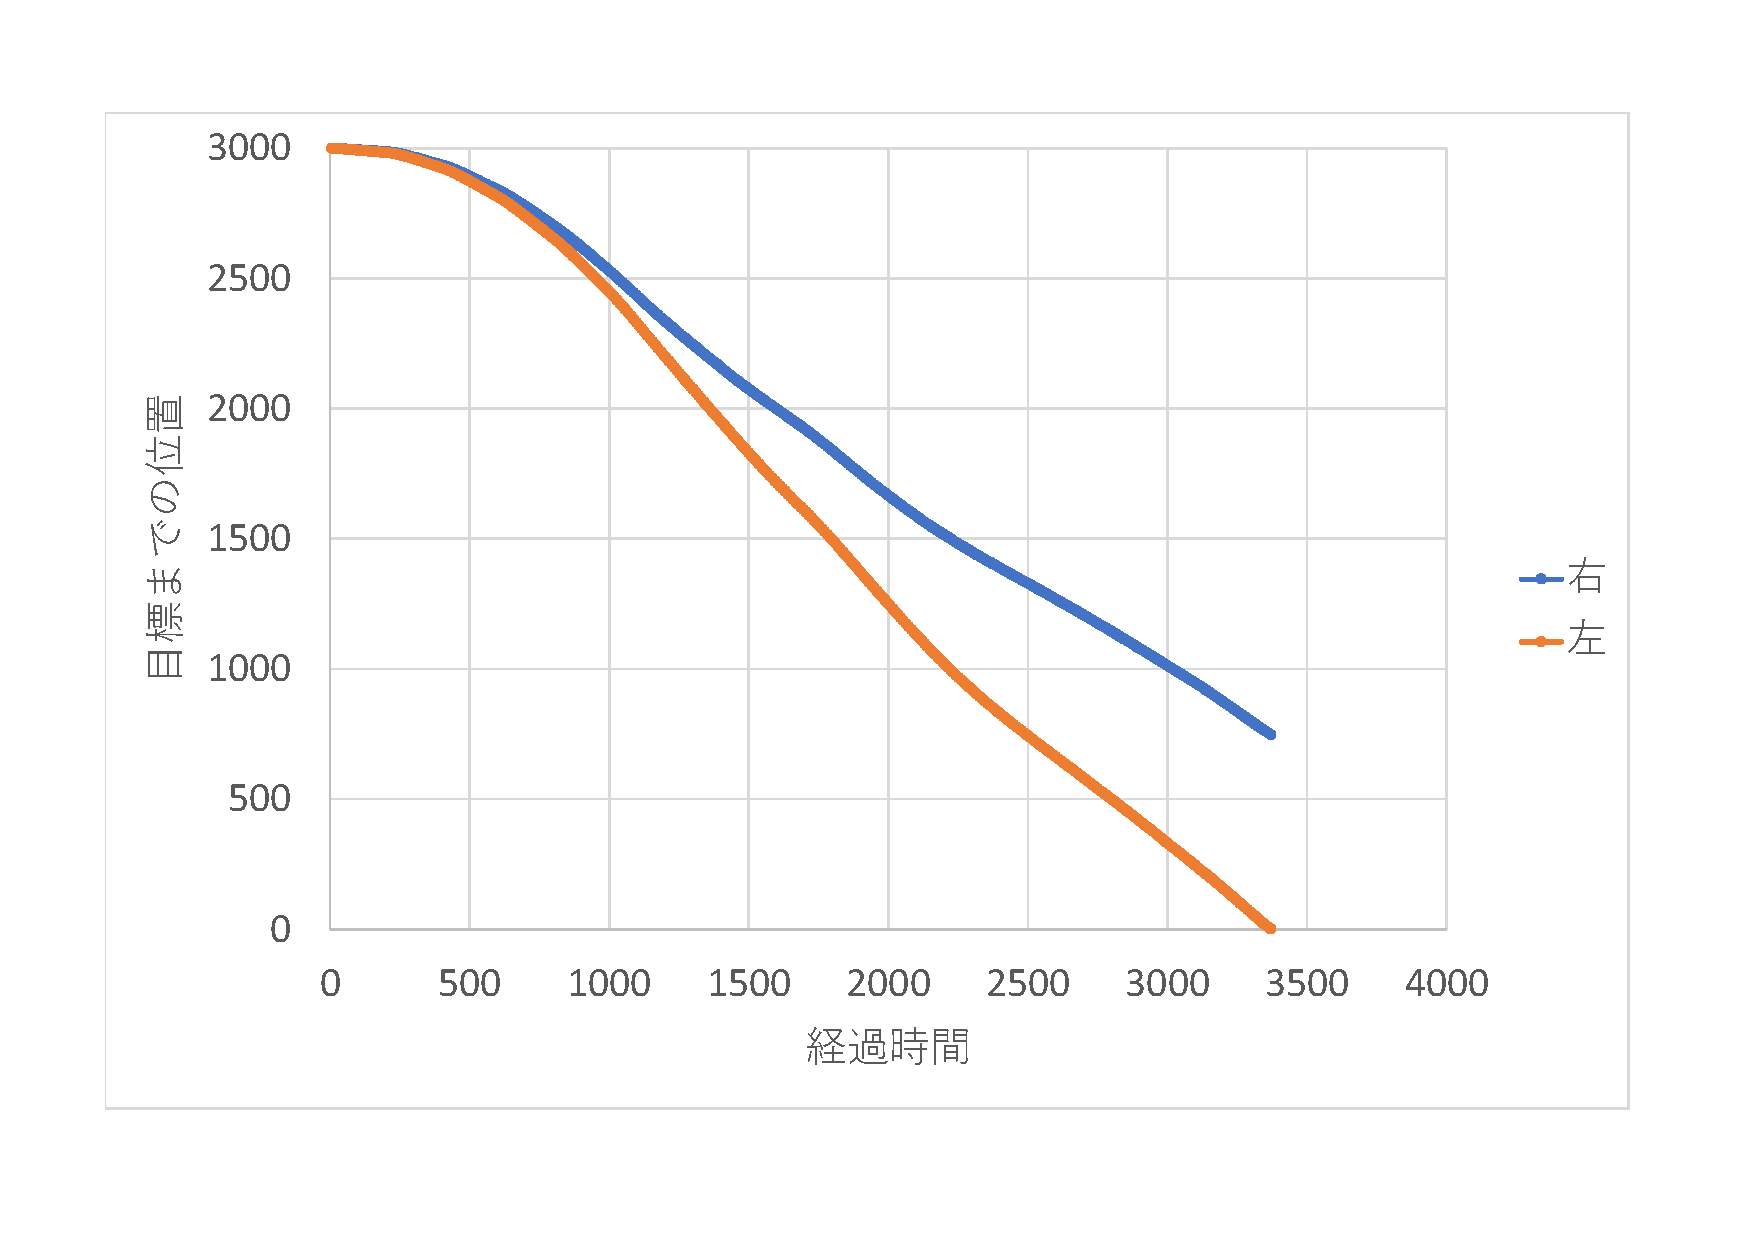
\includegraphics[width=\linewidth]{img/16/16_fuka.pdf}
    }
    \subfigure[負荷無し]{
    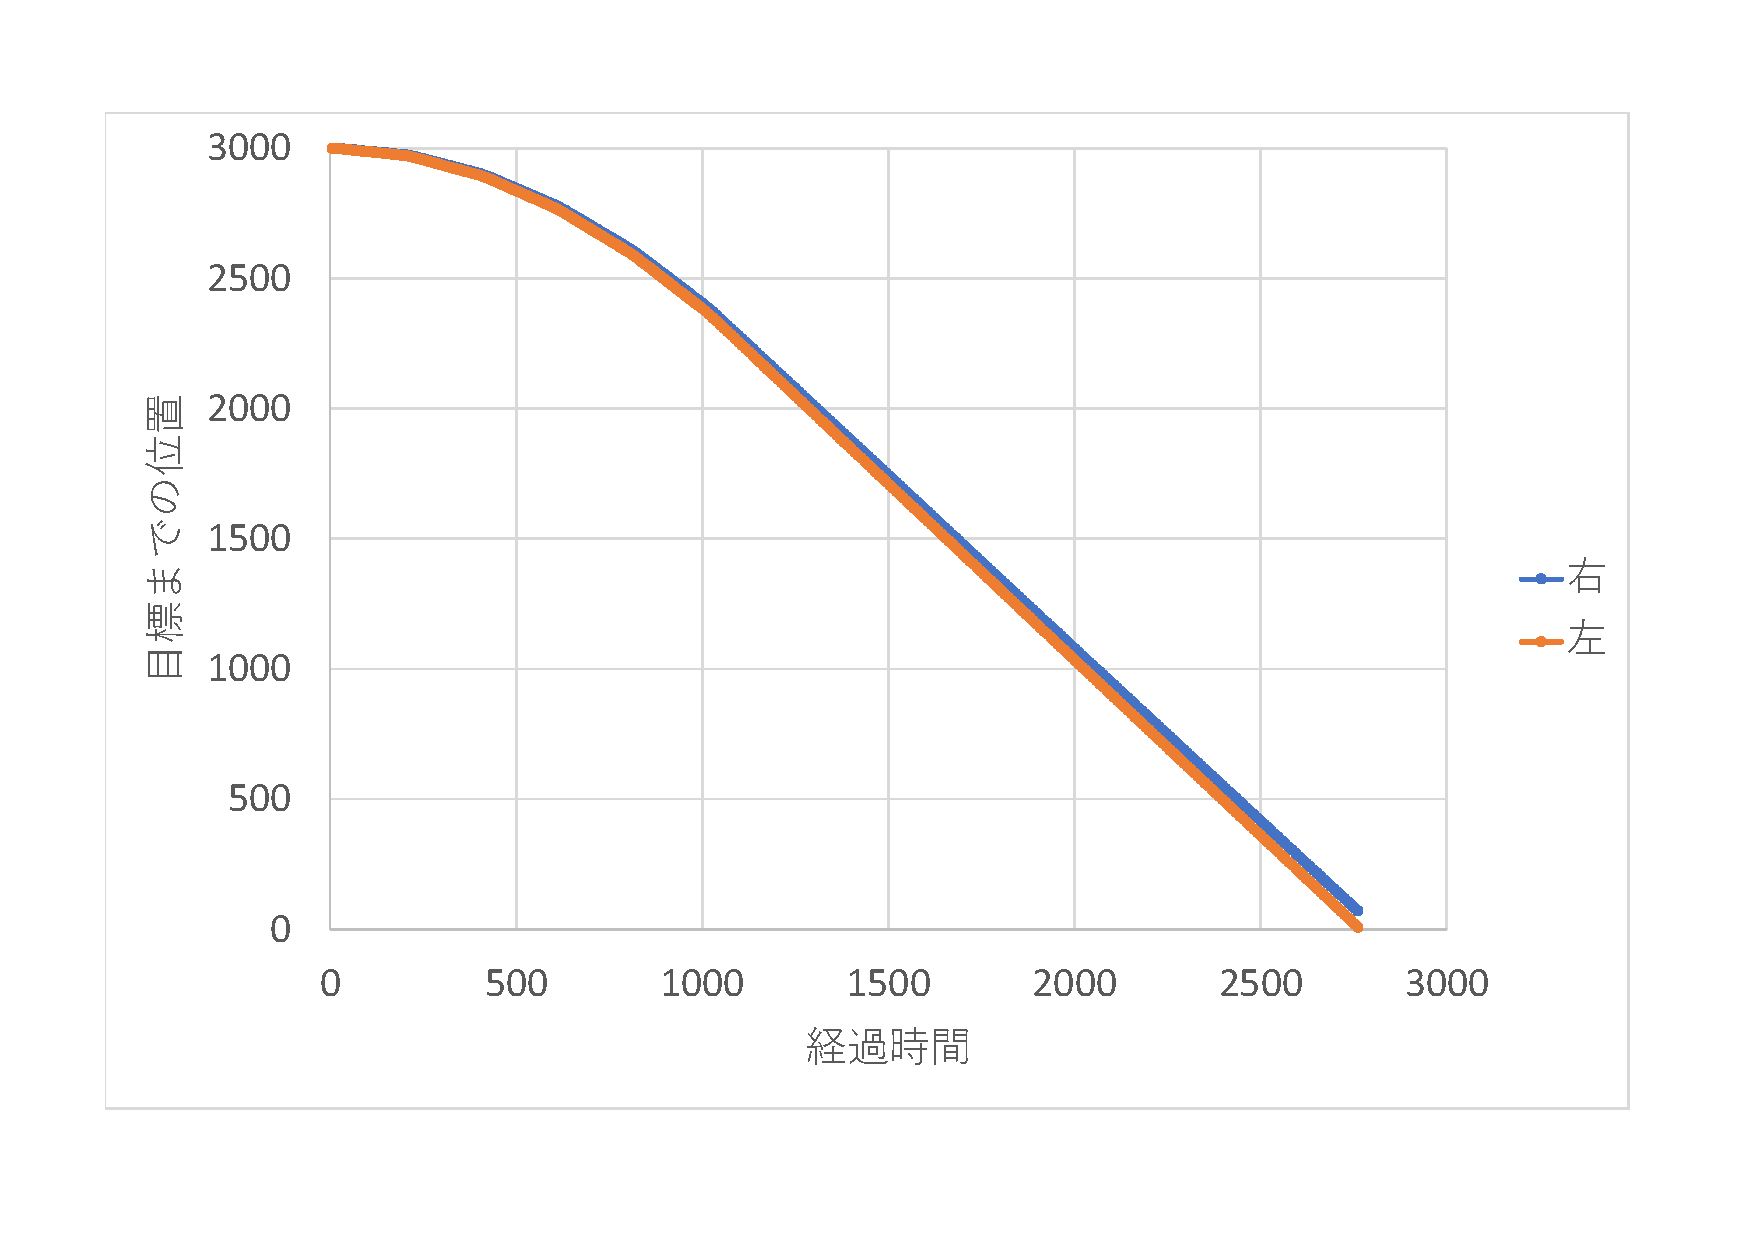
\includegraphics[width=\linewidth]{img/16/16_non.pdf}
    }
  \end{center}
\end{figure}

\section{演習17}
\subsection{実行プログラム}
実行プログラムをソースコード\ref{s17}に示す。
\begin{lstlisting}[caption=演習17のプログラム,label=s17]
#include <stdio.h>
#include <process.h>
#include <dos.h>
#include "v25.h"
#include "ms.h"

#define DMAX 10000
#define INTERVAL 100
#define INTERVAL2 5
#define DISTANCE 3000
#define C_DISTANCE ((DISTANCE*400.*19.225)/(15.*2.*3.14159))
#define THRESH 100
  
int main()
{
    int i, n = 0, n2 = 0;
    double k = ms_read_dip();
    int kp = 3, ki_inv = 10000;
  
    int vref[6] = {1000, 2000, 3000, 4000, 5000, 6000};
    long time[5] = {200, 200, 200, 200, 200};
    long j = 0, cl, cl0, cr, cr0, ct, ct0, ctm, el, er, vl, vr, l[DMAX], r[DMAX], t[DMAX];
    FILE *fp;
  
    ms_init();
    ms_motor_on();
    ms_set_gain( kp, ki_inv );
    ms_read_c( &cl0, &cr0, &ct0 );
    ctm=ct0;
    for( i = 0; i < 5; i++)
    {
        ms_set_v( vref[i], vref[i] );
        do
        {
            ms_read_c( &cl, &cr, &ct );
            n = j/INTERVAL;
            l[n] = cl;
            r[n] = cr;
            t[n] = ct;
            j++;
        } while ( time[i] > ct-ctm );
        ctm = ct;
    }
    j = 0;
    do
    {
        el = C_DISTANCE - cl;
        er = C_DISTANCE - cr;
        vl = k * el;
        vr = k * er;
        if ( vl > vref[5] )
        {
            vl = vref[5];
        }
        if ( vr > vref[5] )
        {
            vr = vref[5];
        }
        ms_set_v( vl, vr );
        ms_read_c( &cl, &cr, &ct );
        n2 = j/INTERVAL2 + n + 1;
        l[n2] = cl;
        r[n2] = cr;
        t[n2] = ct;
        j++; 
    } while ( n2<DMAX && el>THRESH && er>THRESH );
      
    ms_motor_off();
  
    if ((fp = fopen("data.dat","wt")) == NULL)
    {
        printf("Can't open file.\n");
        exit(1);
    }

    for ( i = 0; i < n2; i++)
    {
        fprintf(fp,"%12.6lf %12.6lf %5ld\n",DISTANCE-15*2*3.14159*(l[i]-cl0)/(19.225*400),DISTANCE-15*2*3.14159*(r[i]-cr0)/(19.225*400),t[i]-ct0);
    }
    fclose(fp);
  
    printf("owari\n");
    ms_beep(440,500);
    return 0;
}
\end{lstlisting}
\mysubsection{実行結果}
実行結果を図\ref{im32}から\ref{im41}に示す。
$k = 1$において、ロボットが目標位置に到着した際に転倒し、
距離データの記録が5000秒付近まで続いている。

また、負荷有りよりも負荷無しの方が、目標位置への所要時間が少ない。
位置のフィードバックゲインの値を大きくすると、目標位置までの所要時間が減少する。


\begin{figure}
  \begin{center}
  \subfigure[$k=1$ 負荷有り]{
  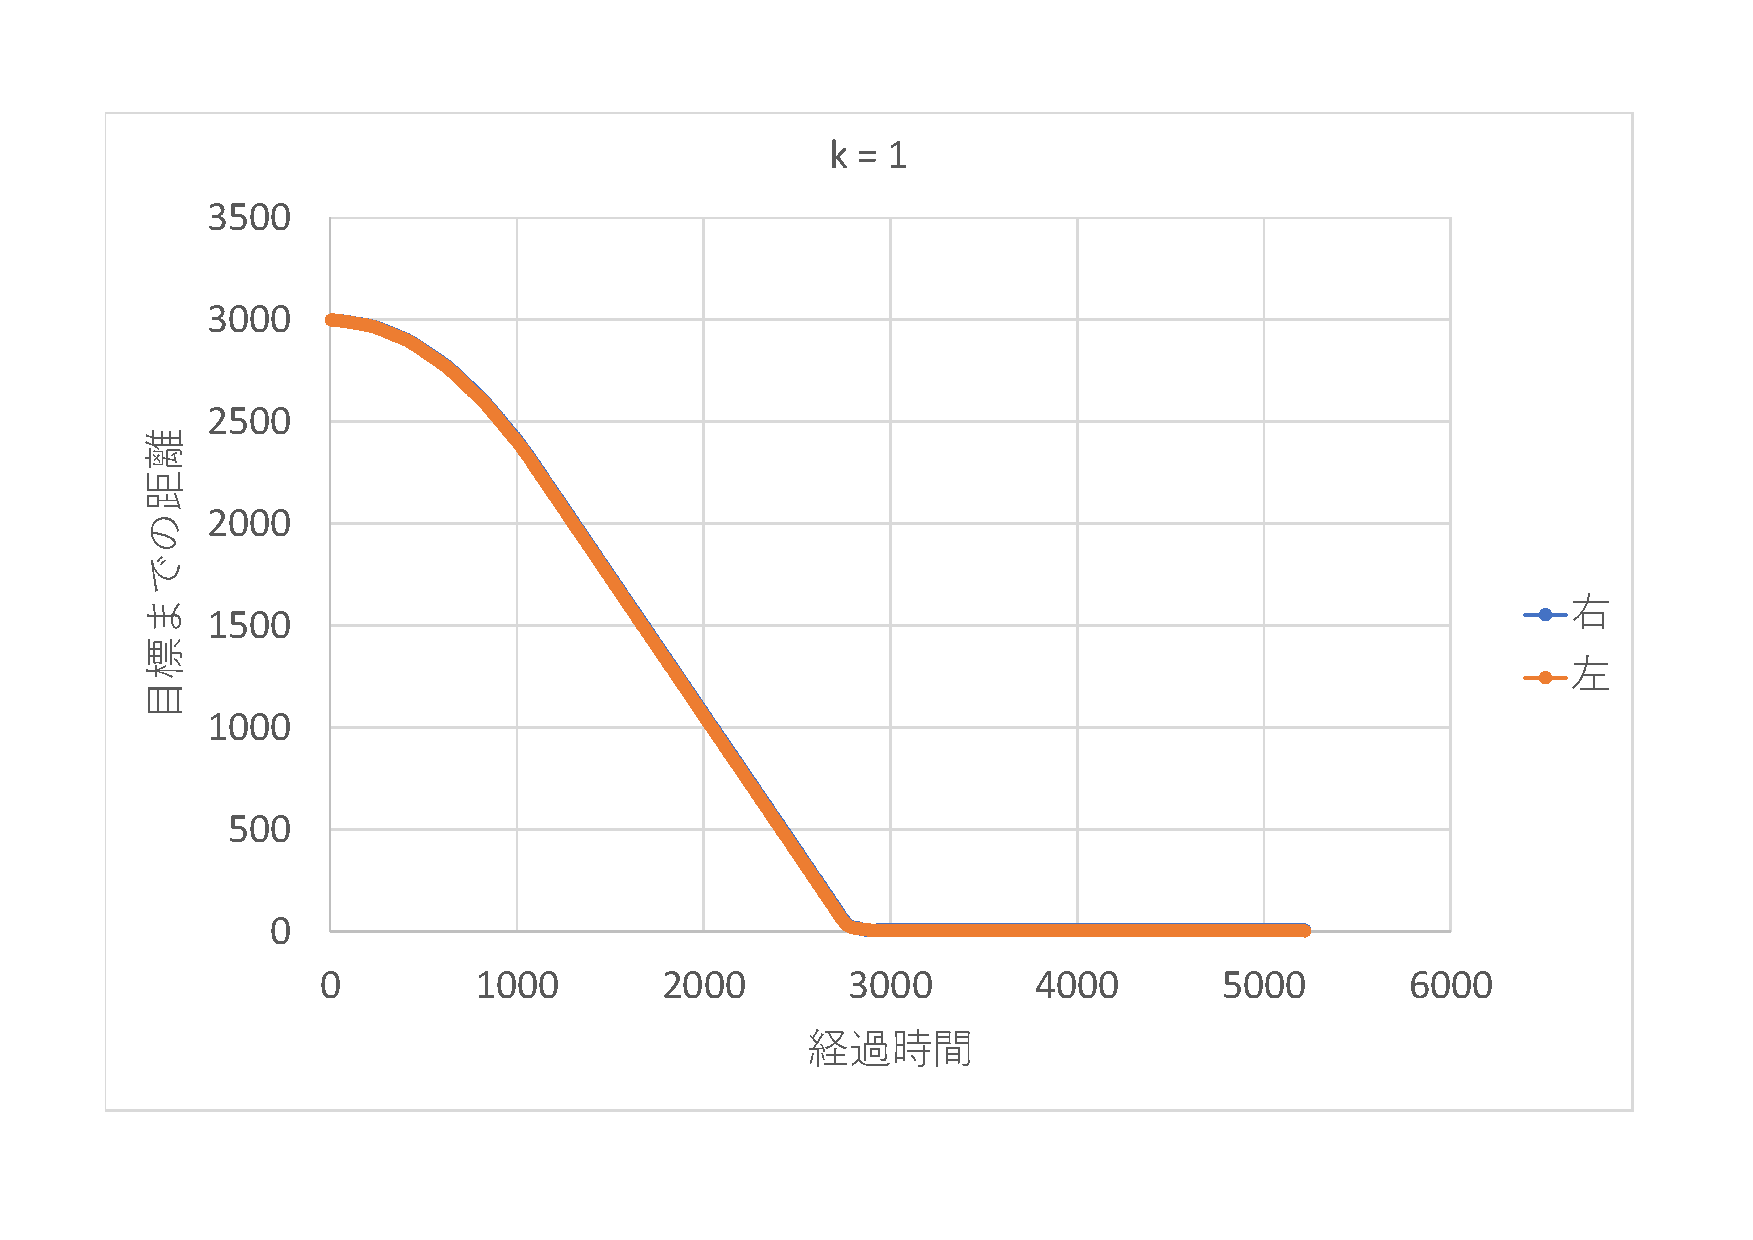
\includegraphics[width=\linewidth]{img/17/17_fuka_K1.pdf}
  \label{im32}
  }
  \subfigure[$k=1$ 負荷無し]{
  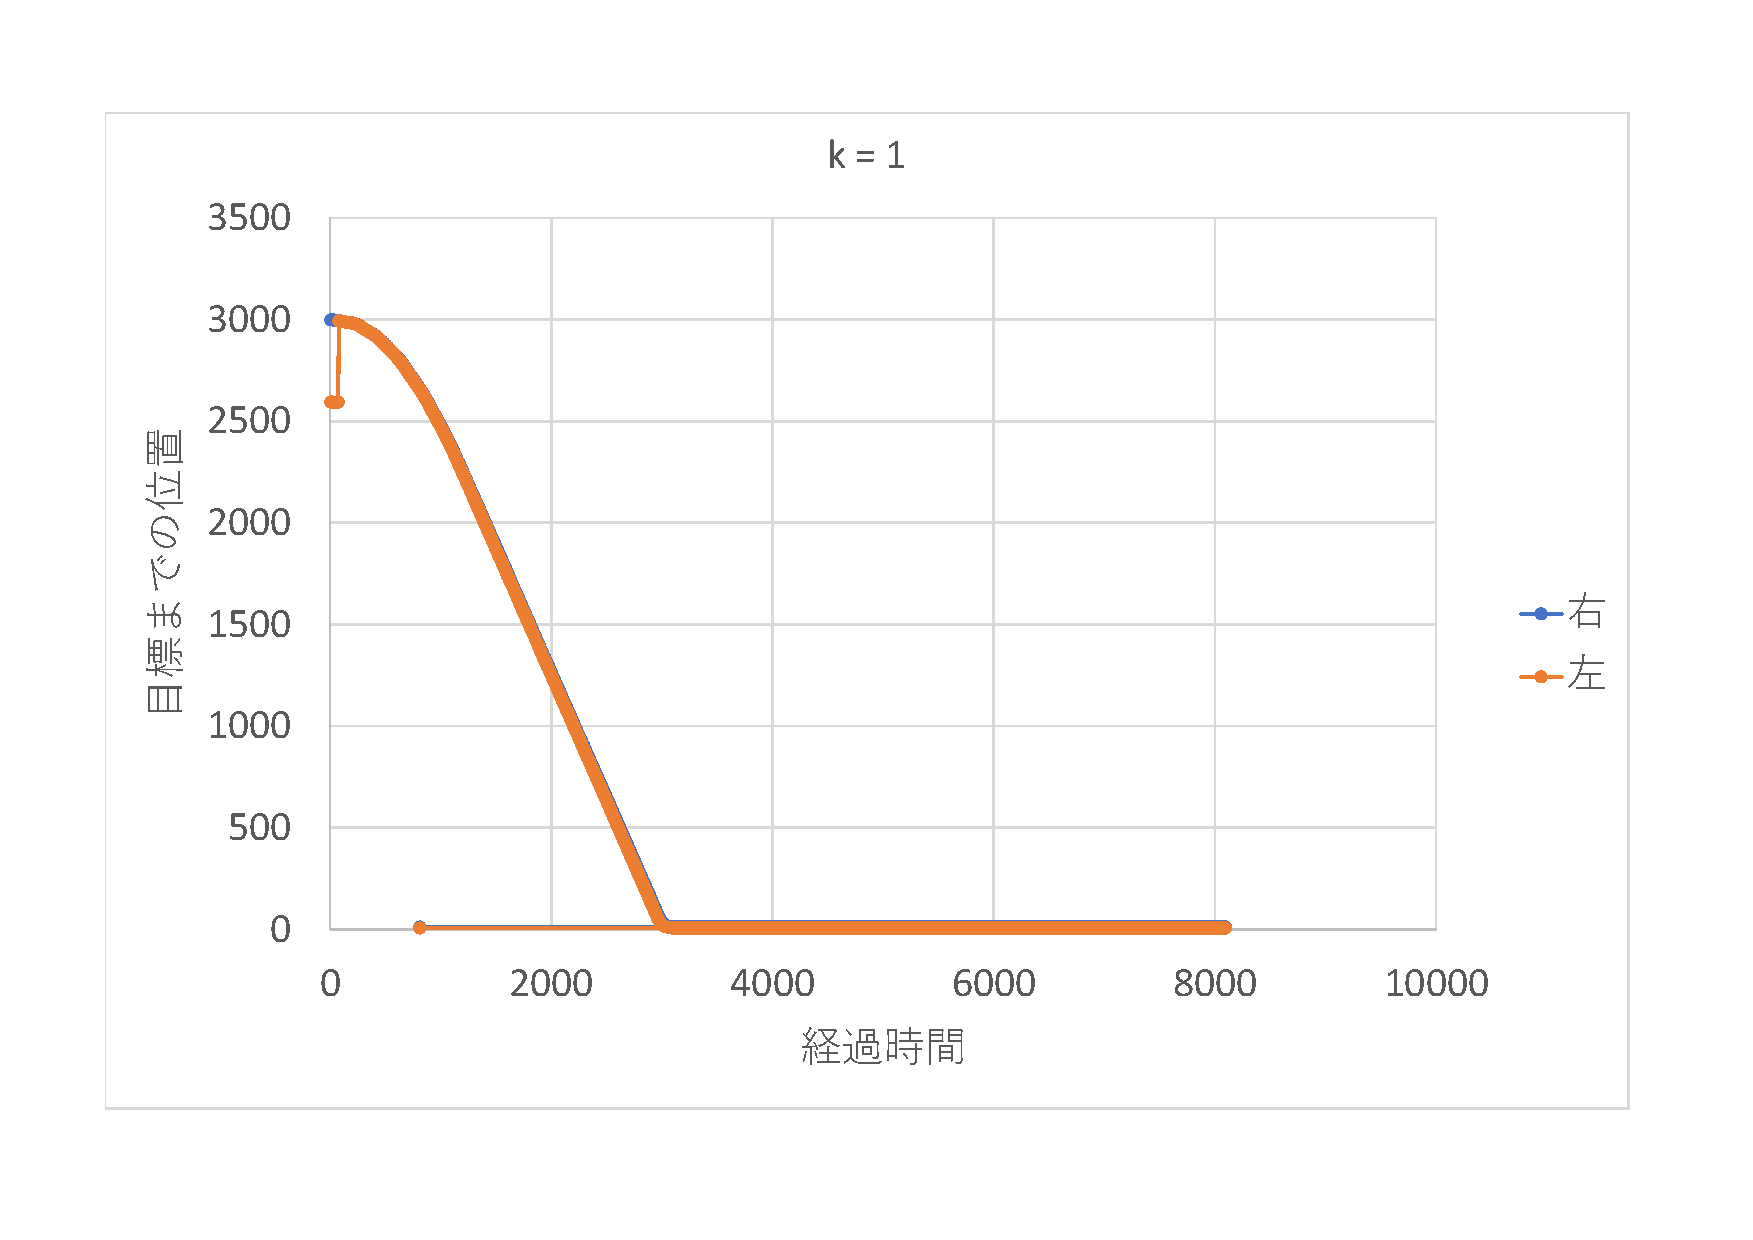
\includegraphics[width=\linewidth]{img/17/17_non_K1.pdf}
  \label{im33}
  }
  \caption{$k = 1$のステップ応答}
  \end{center}
\end{figure}

\begin{figure}
  \begin{center}
  \subfigure[$k=2$ 負荷有り]{
  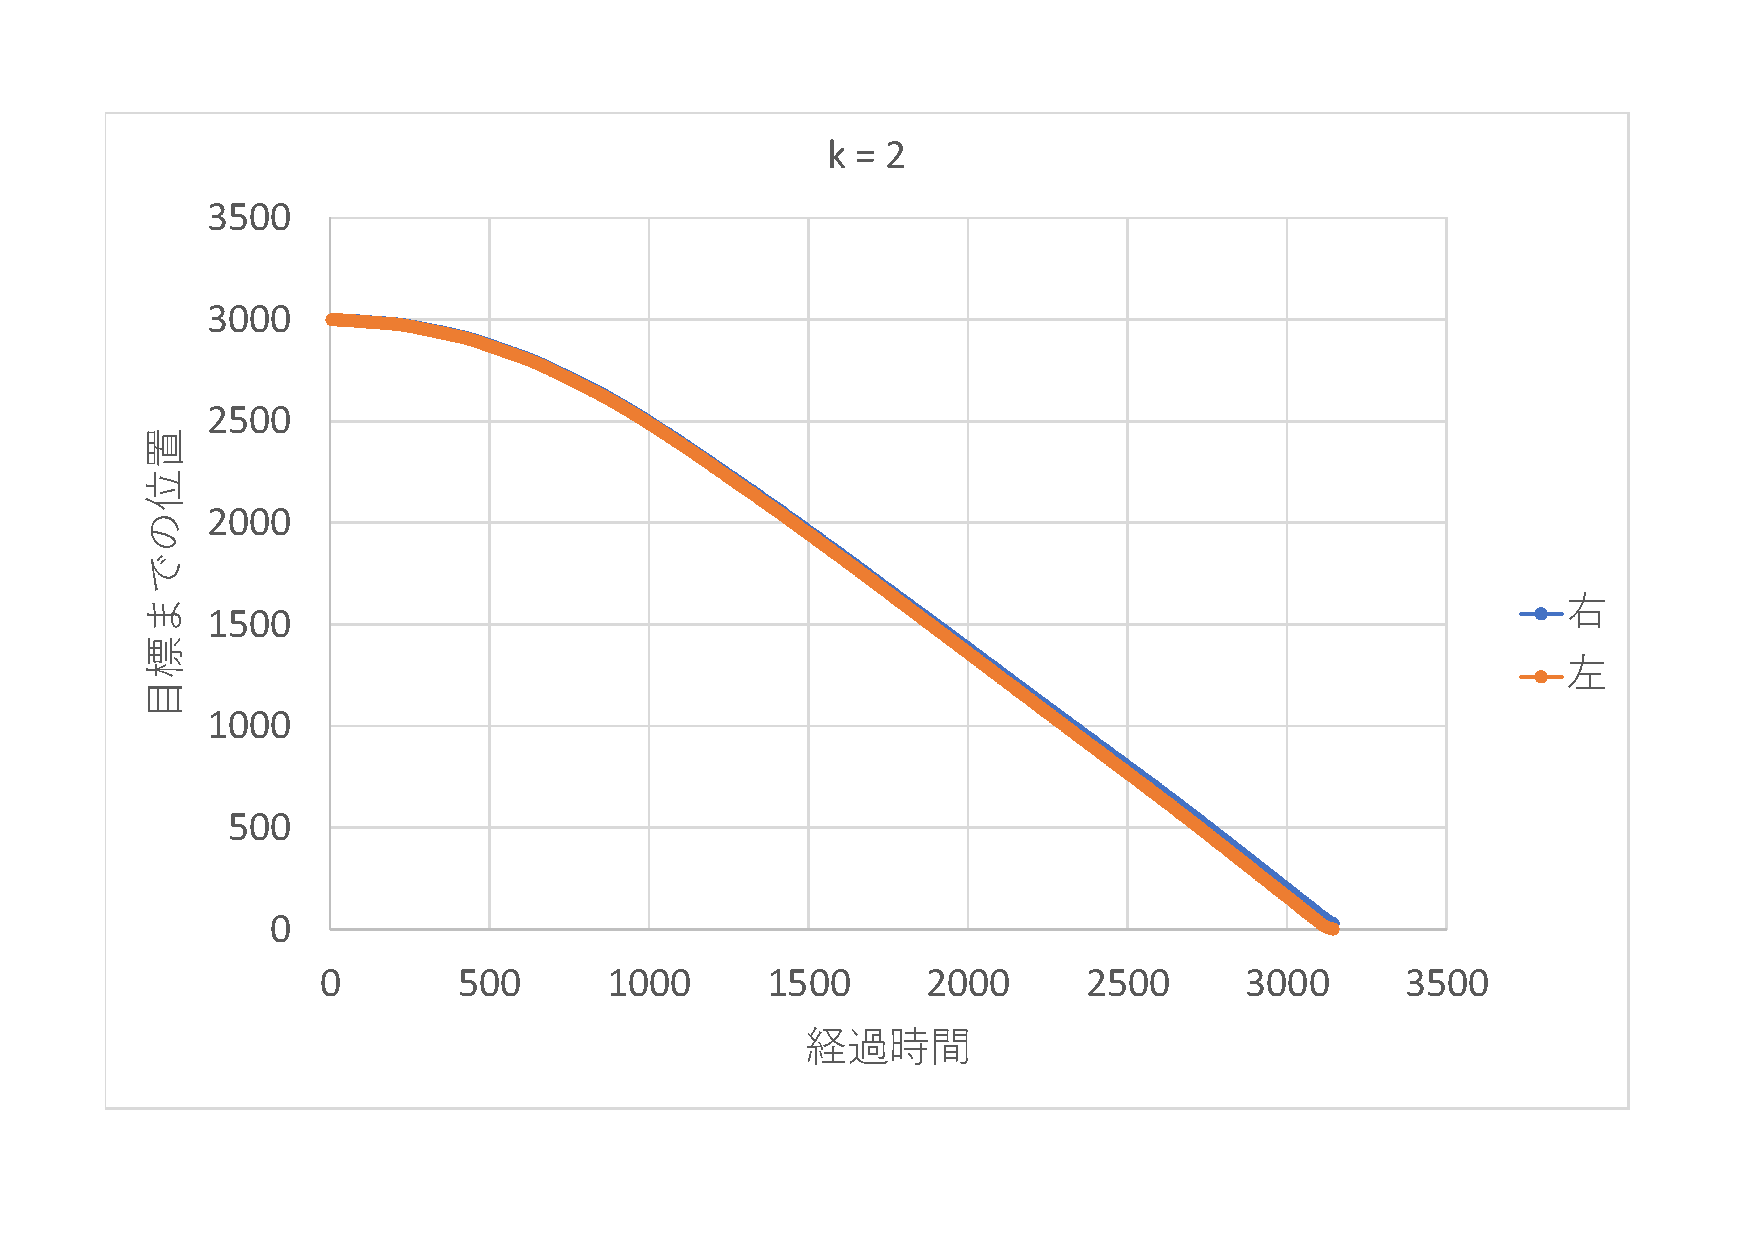
\includegraphics[width=\linewidth]{img/17/17_fuka_K2.pdf}
  \label{im34}
  }
  \subfigure[$k=2$ 負荷無し]{
  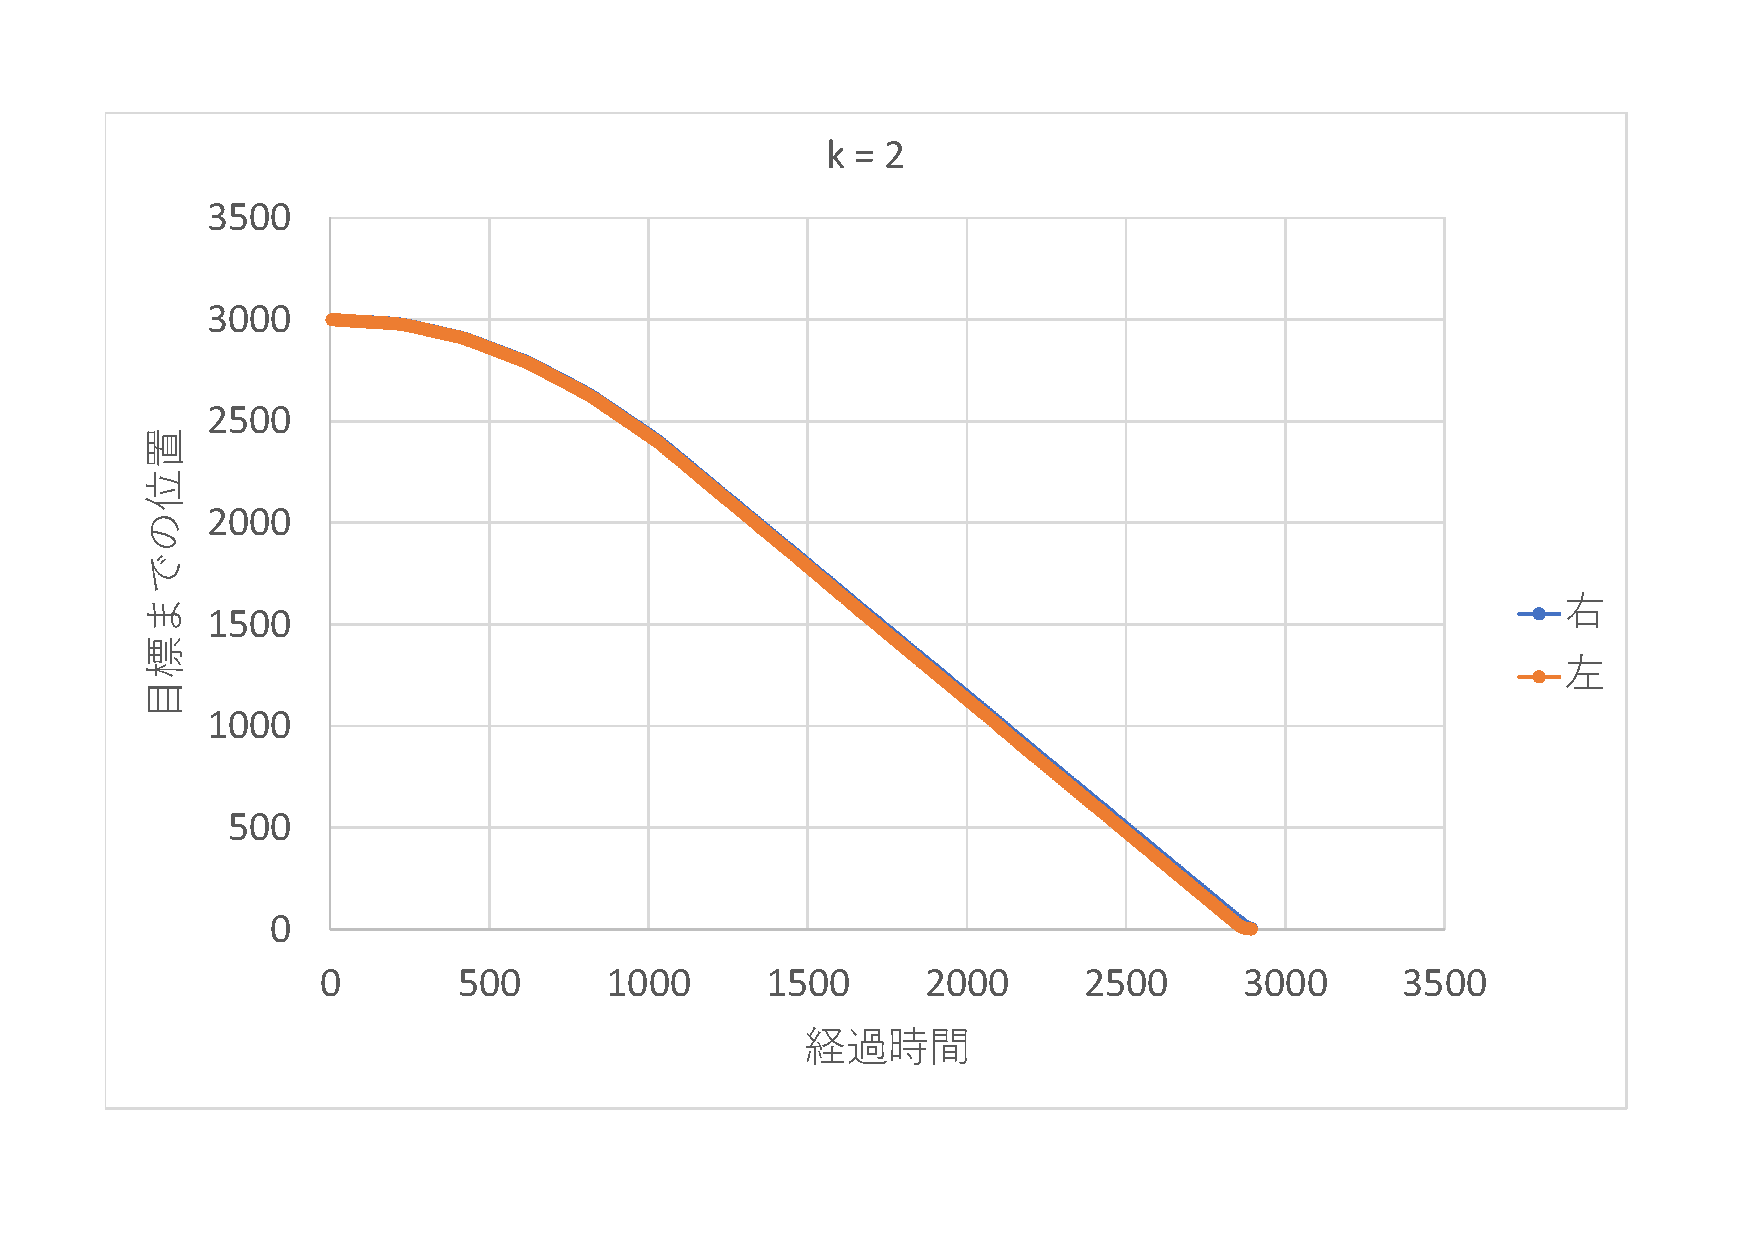
\includegraphics[width=\linewidth]{img/17/17_non_K2.pdf}
  \label{im35}
  }
  \caption{$k=2$のステップ応答}
  \end{center}
\end{figure}

\begin{figure}
  \begin{center}
  \subfigure[$k=3$ 負荷有り]{
  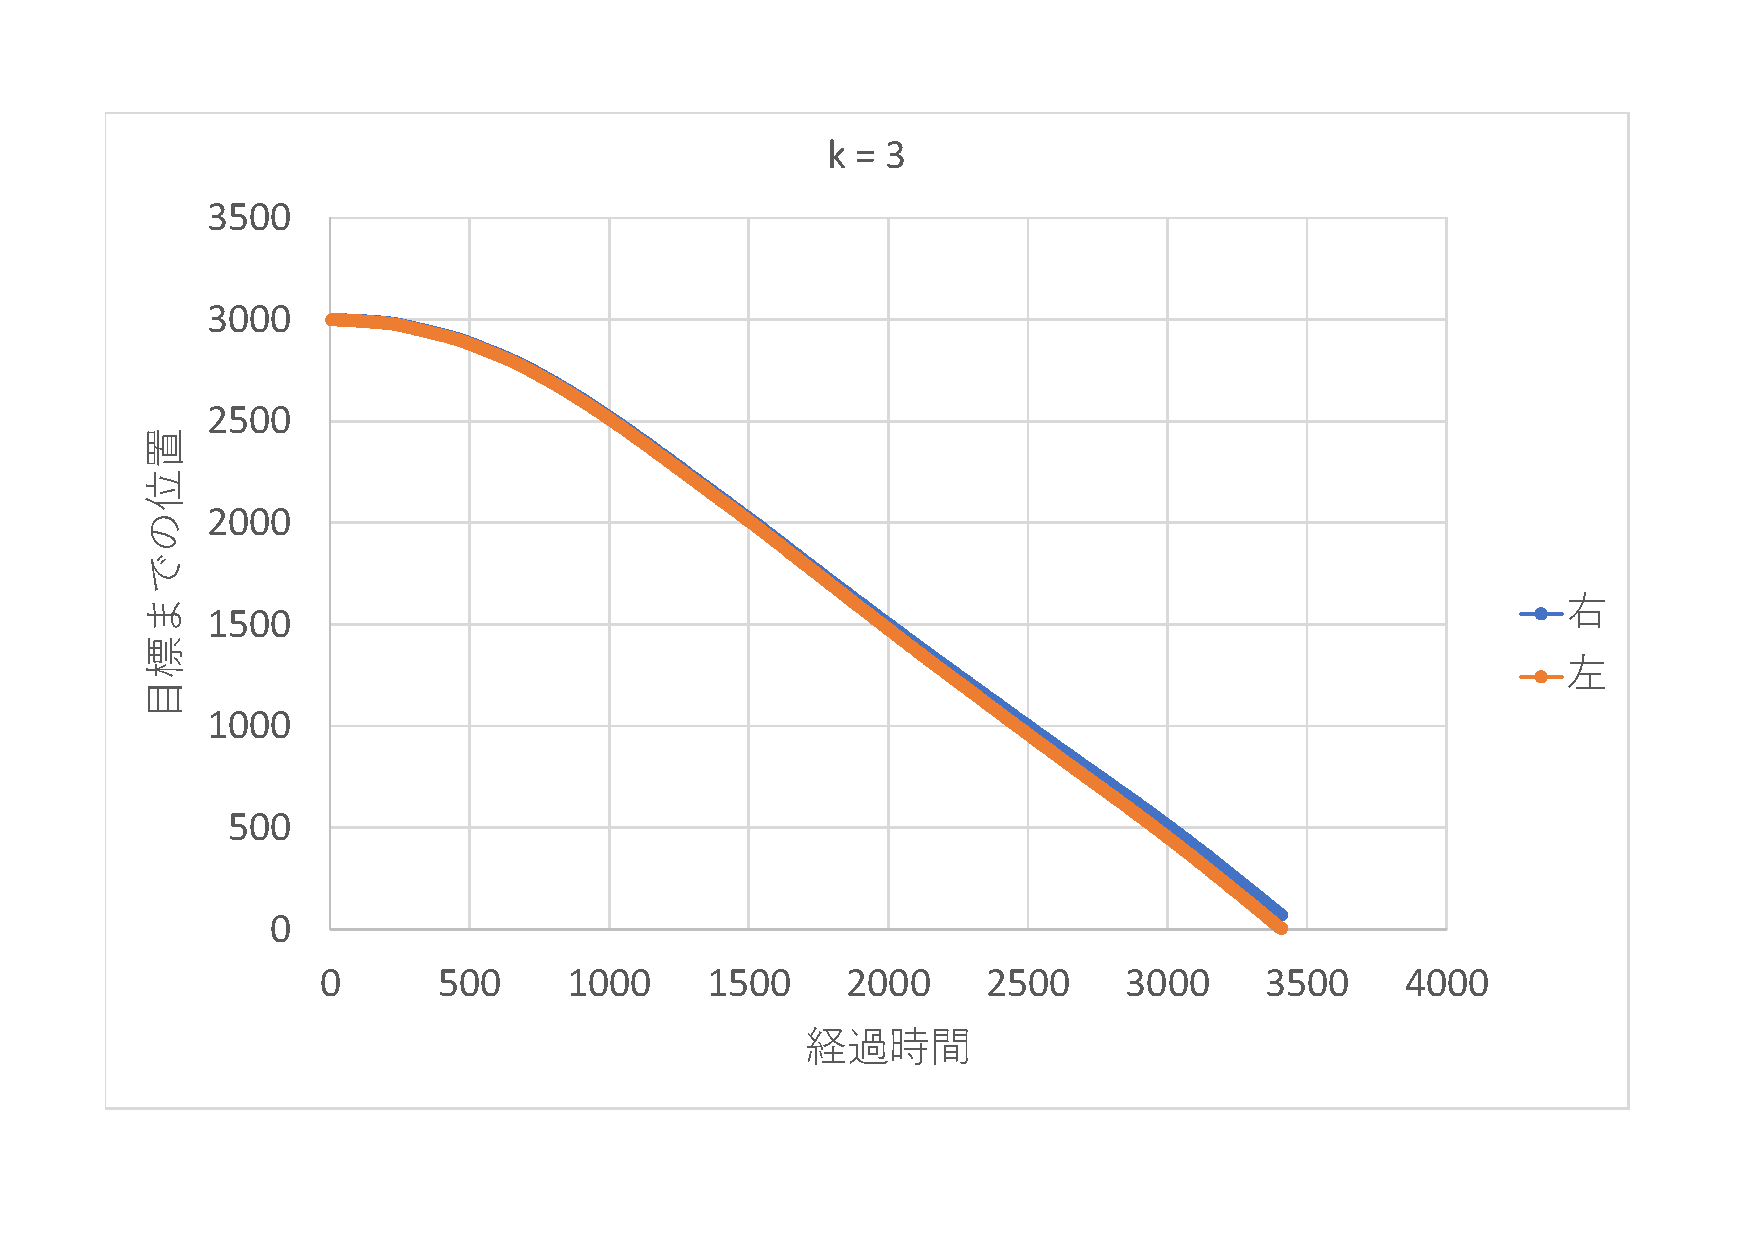
\includegraphics[width=\linewidth]{img/17/17_fuka_K3.pdf}
  \label{im36}
  }
  \subfigure[$k=3$ 負荷無し]{
  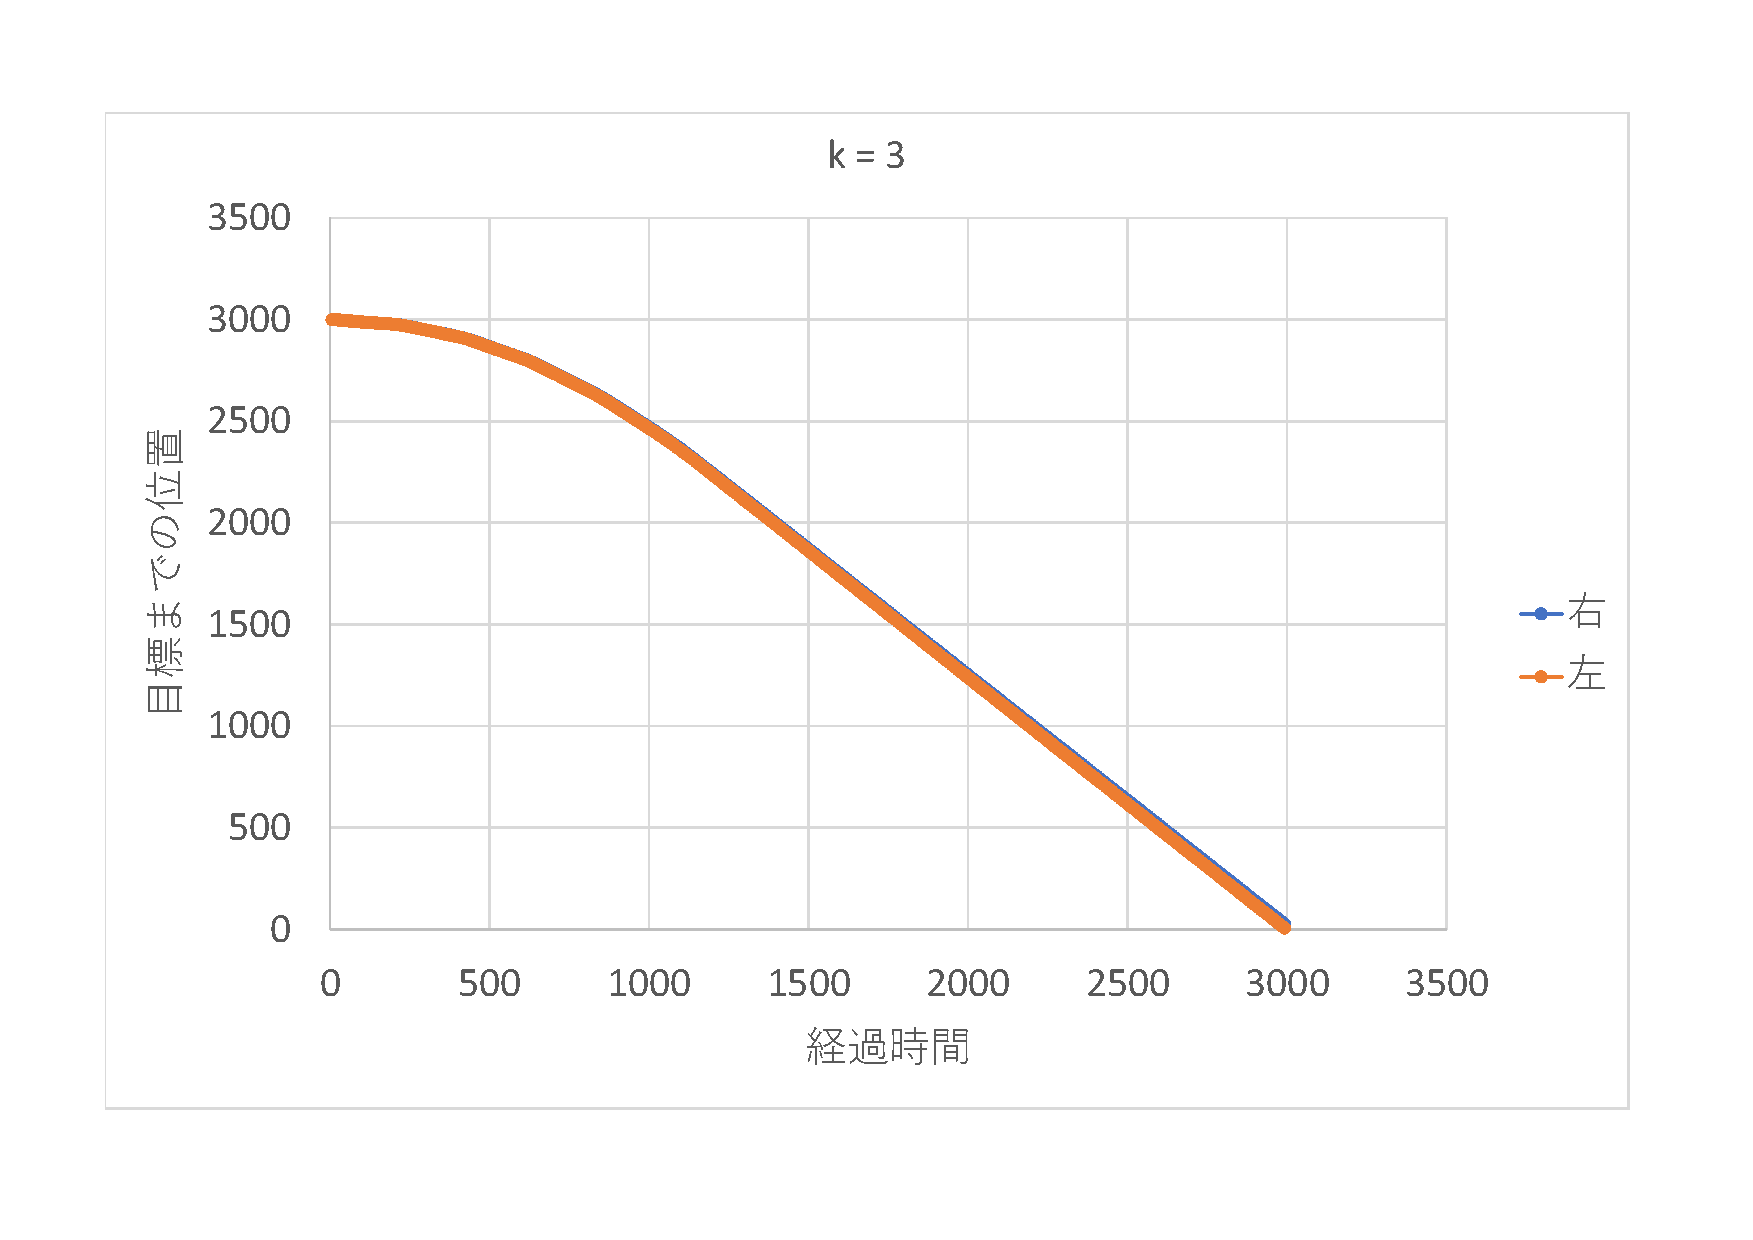
\includegraphics[width=\linewidth]{img/17/17_non_K3.pdf}
  \label{im37}
  }
  \caption{$k=3$のステップ応答}
  \end{center}
\end{figure}

\begin{figure}
  \begin{center}
  \subfigure[$k=6$ 負荷有り]{
  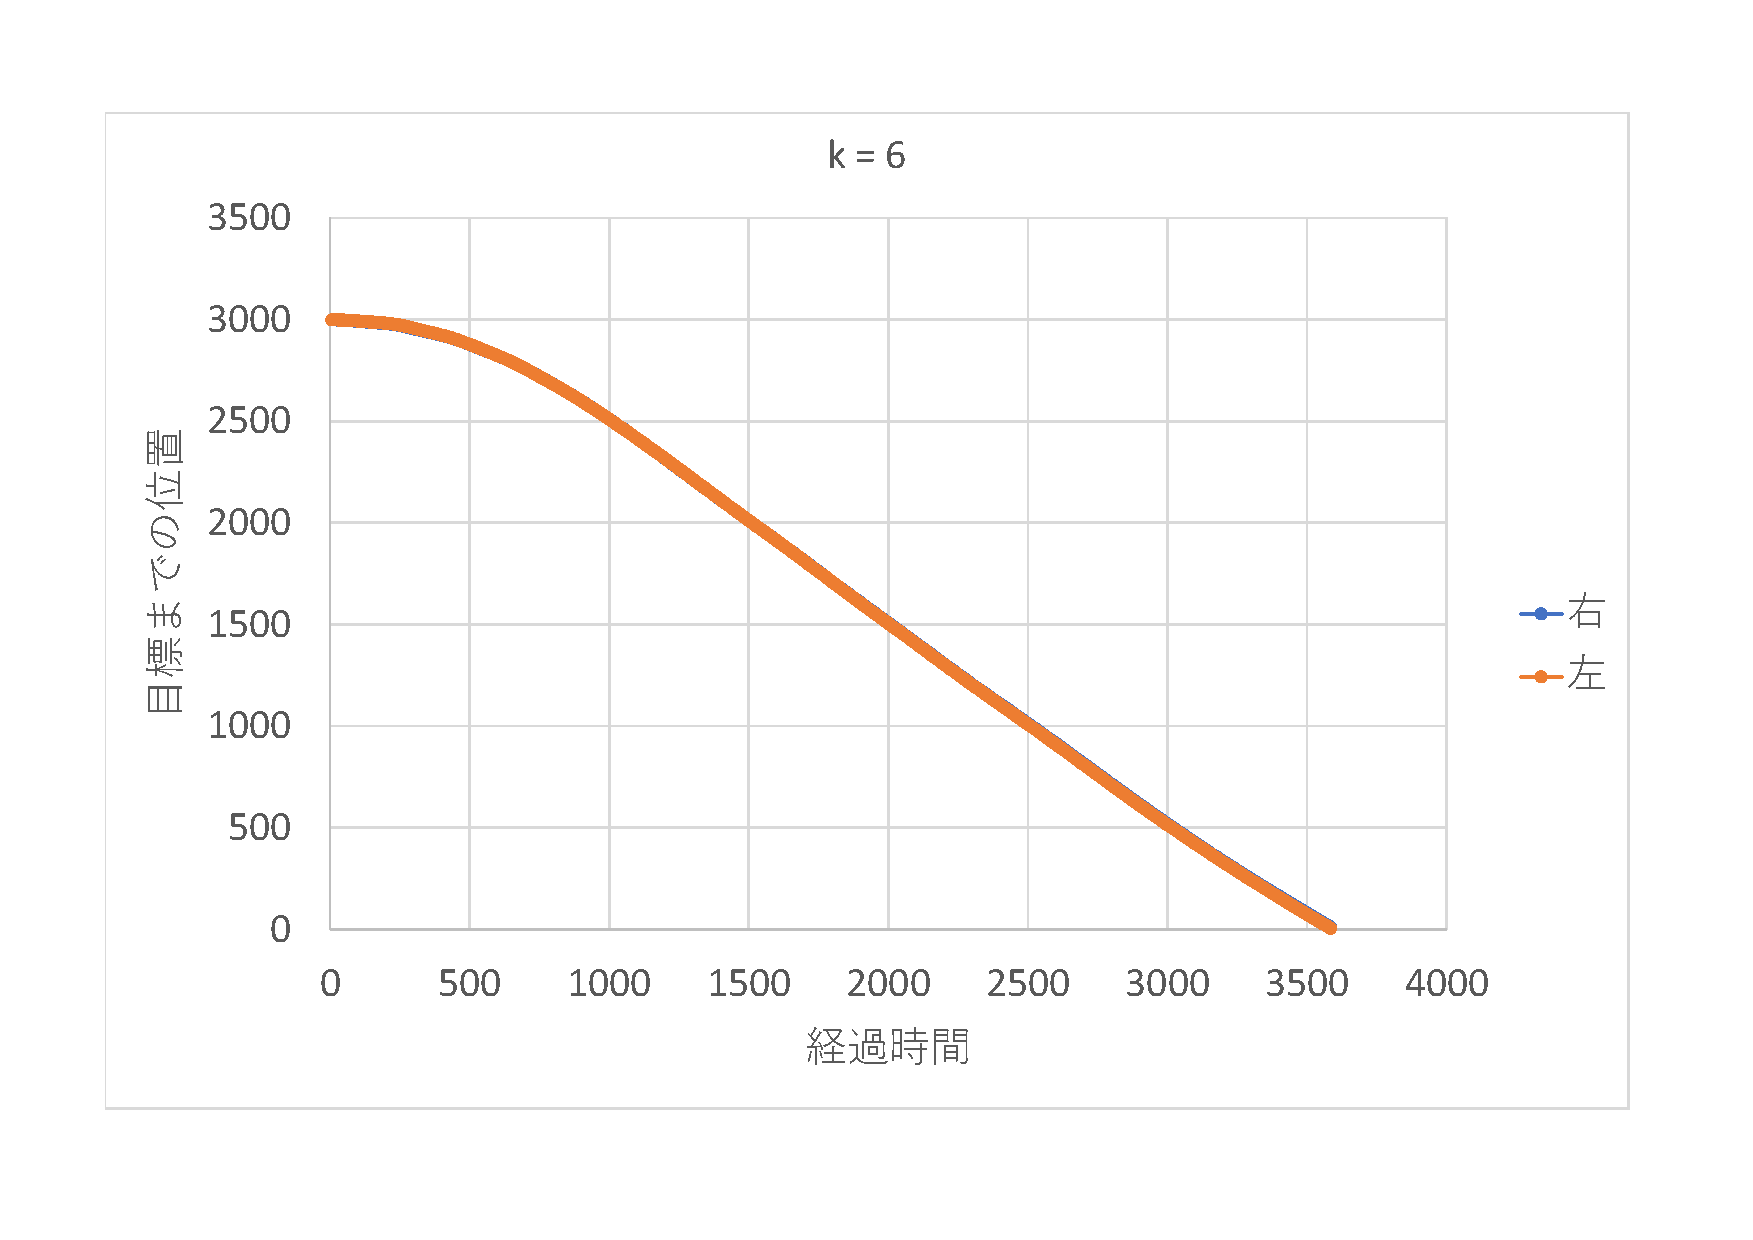
\includegraphics[width=\linewidth]{img/17/17_fuka_K6.pdf}
  \label{im38}
  }
  \subfigure[$k=6$ 負荷無し]{
  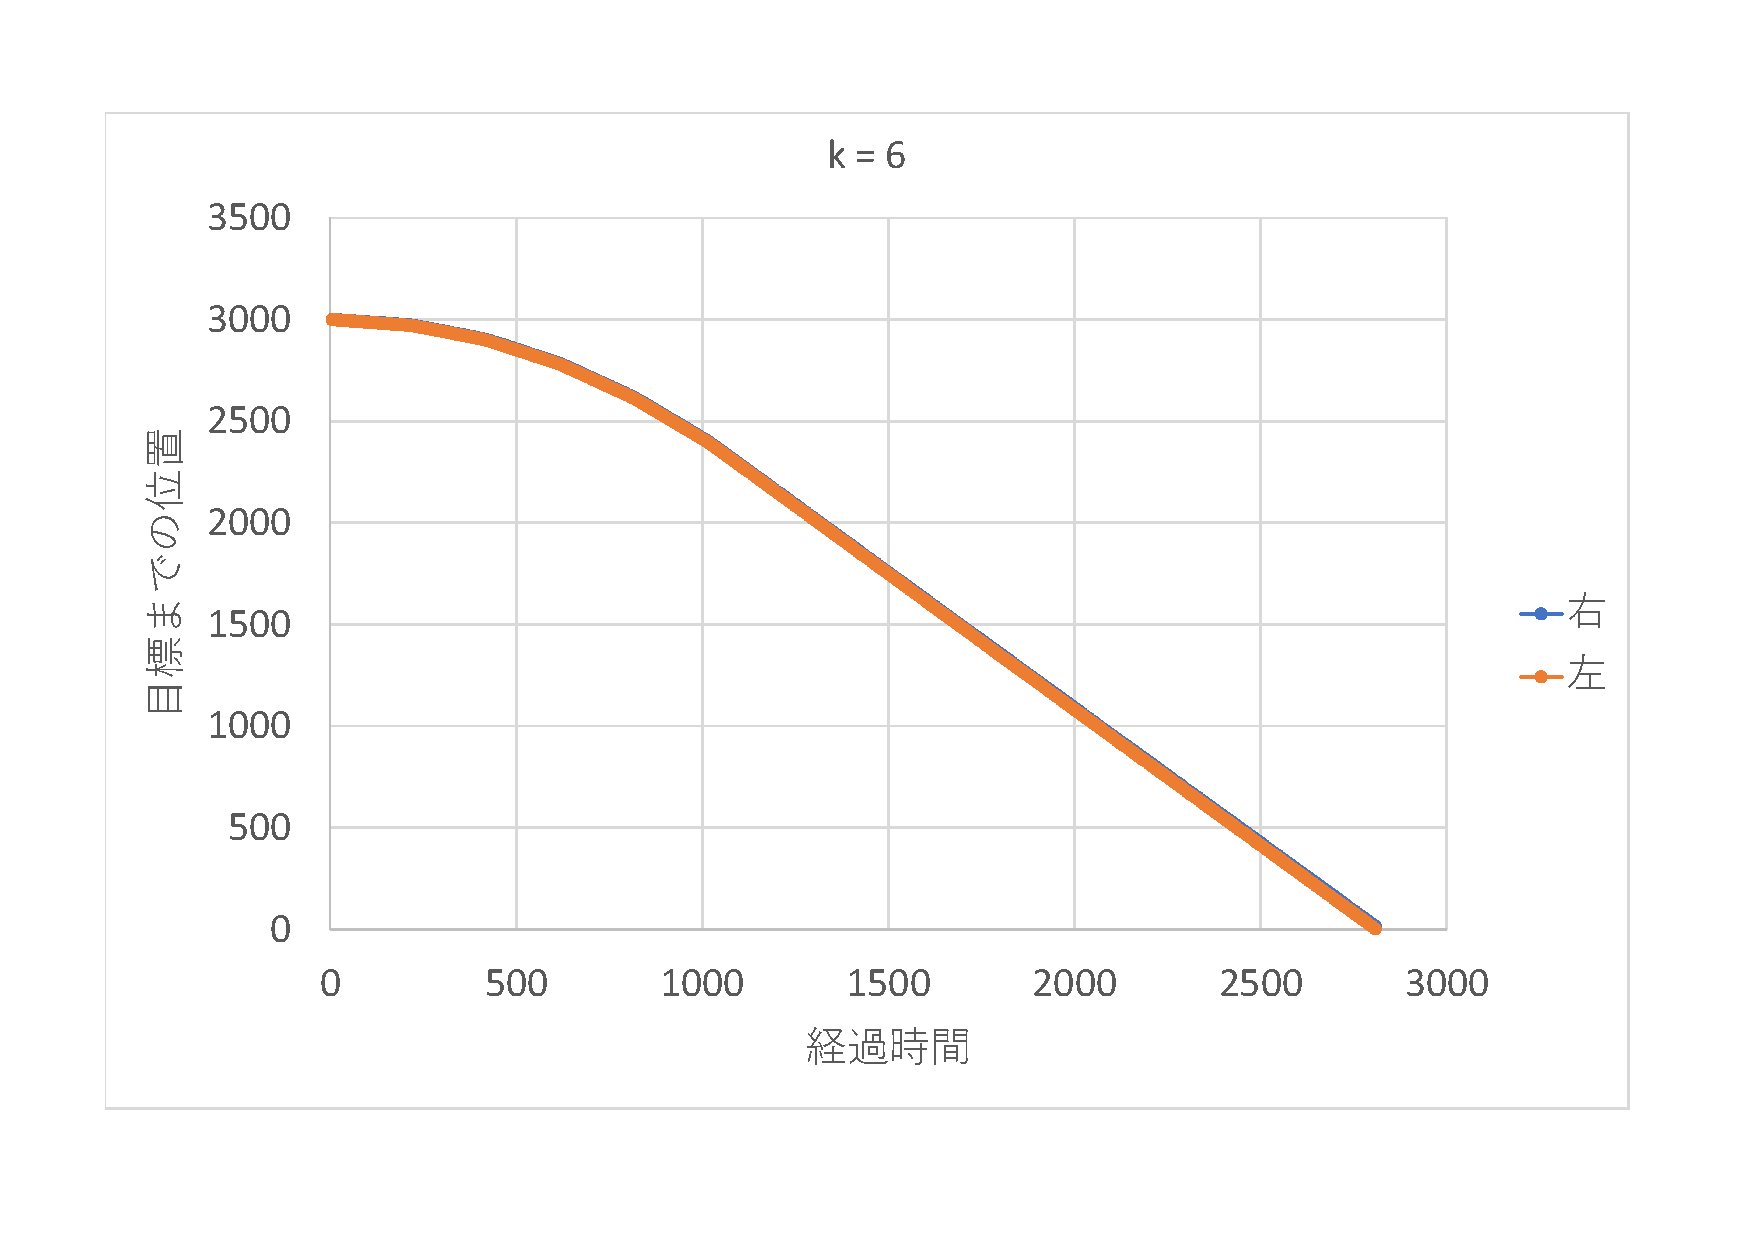
\includegraphics[width=\linewidth]{img/17/17_non_K6.pdf}
  \label{im39}
  }
  \caption{$k=6$のステップ応答}
  \end{center}
\end{figure}

\begin{figure}
  \begin{center}
  \subfigure[$k=10$ 負荷有り]{
  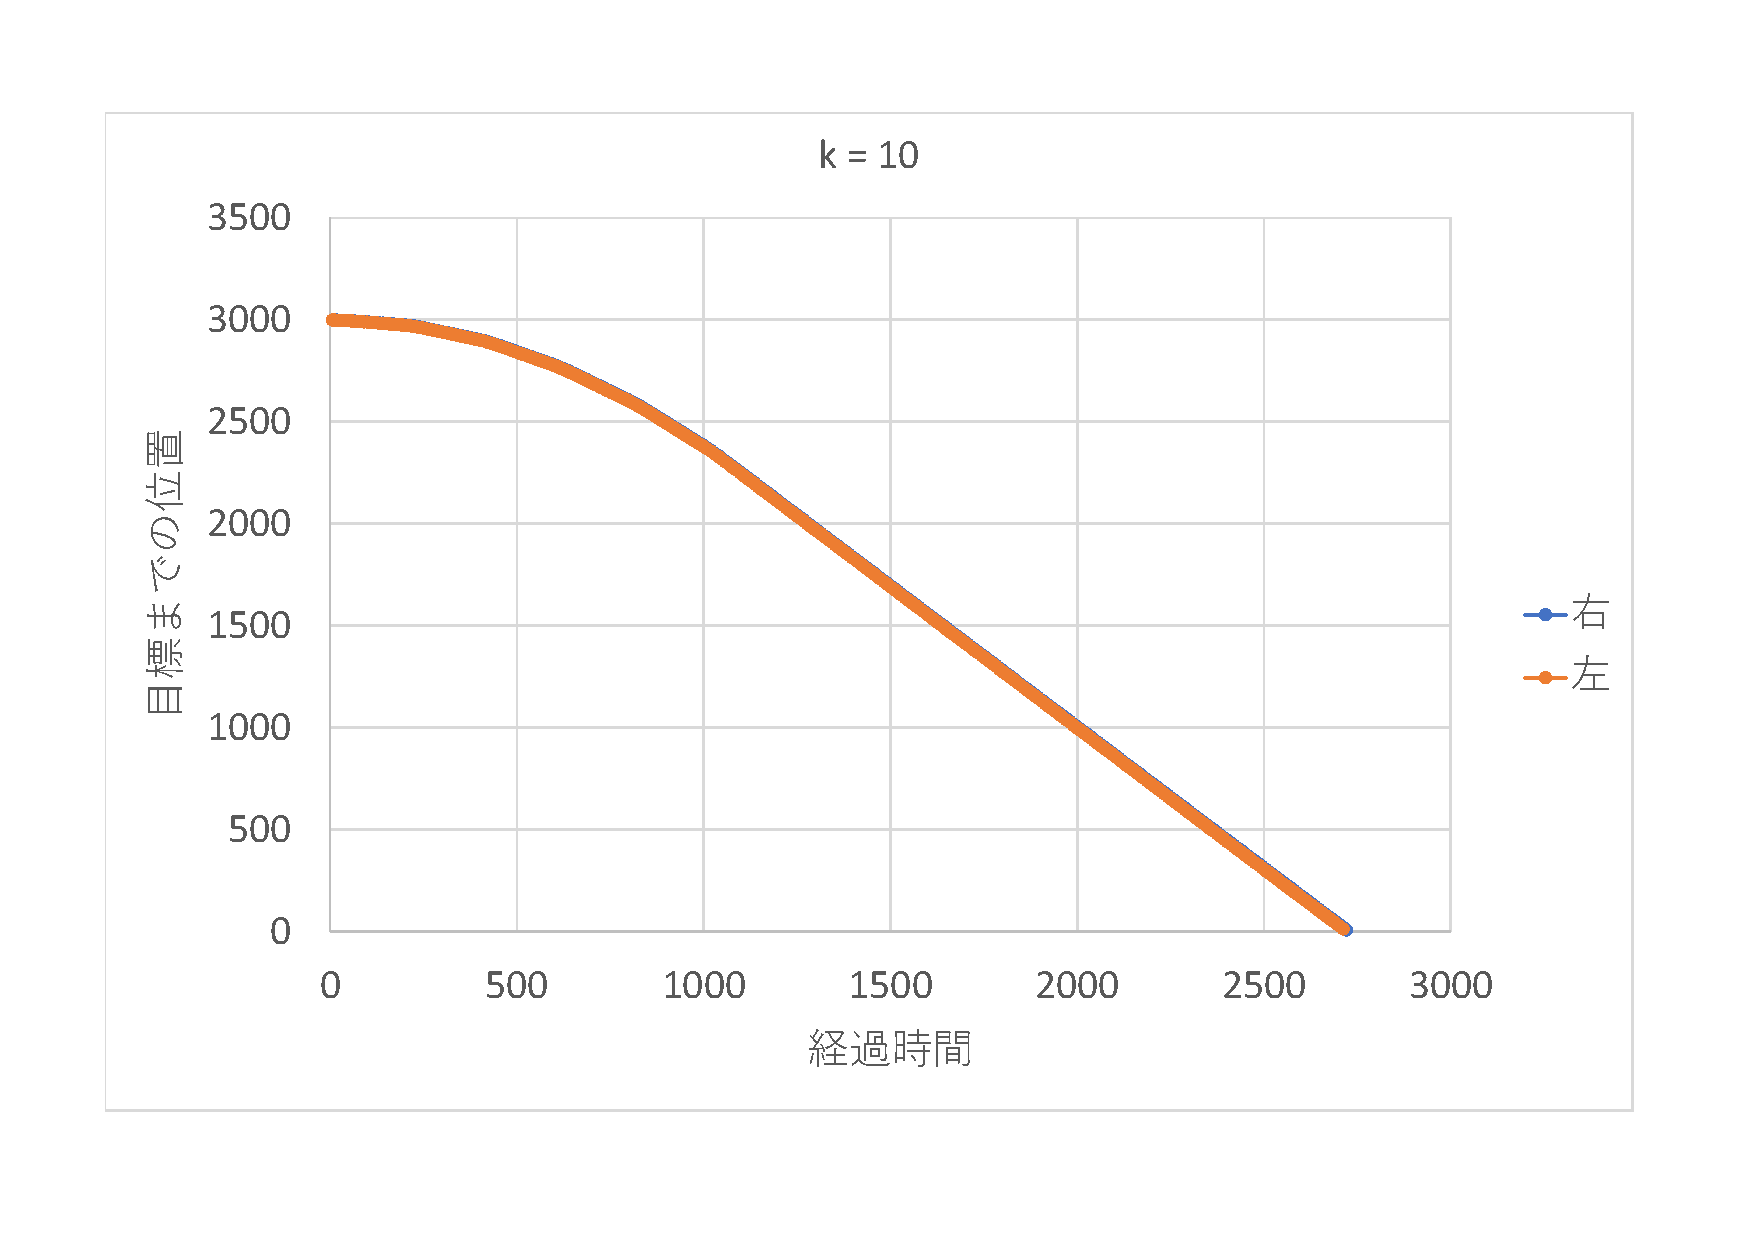
\includegraphics[width=\linewidth]{img/17/17_fuka_K10.pdf}
  \label{im40}
  }
  \subfigure[$k=10$ 負荷無し]{
  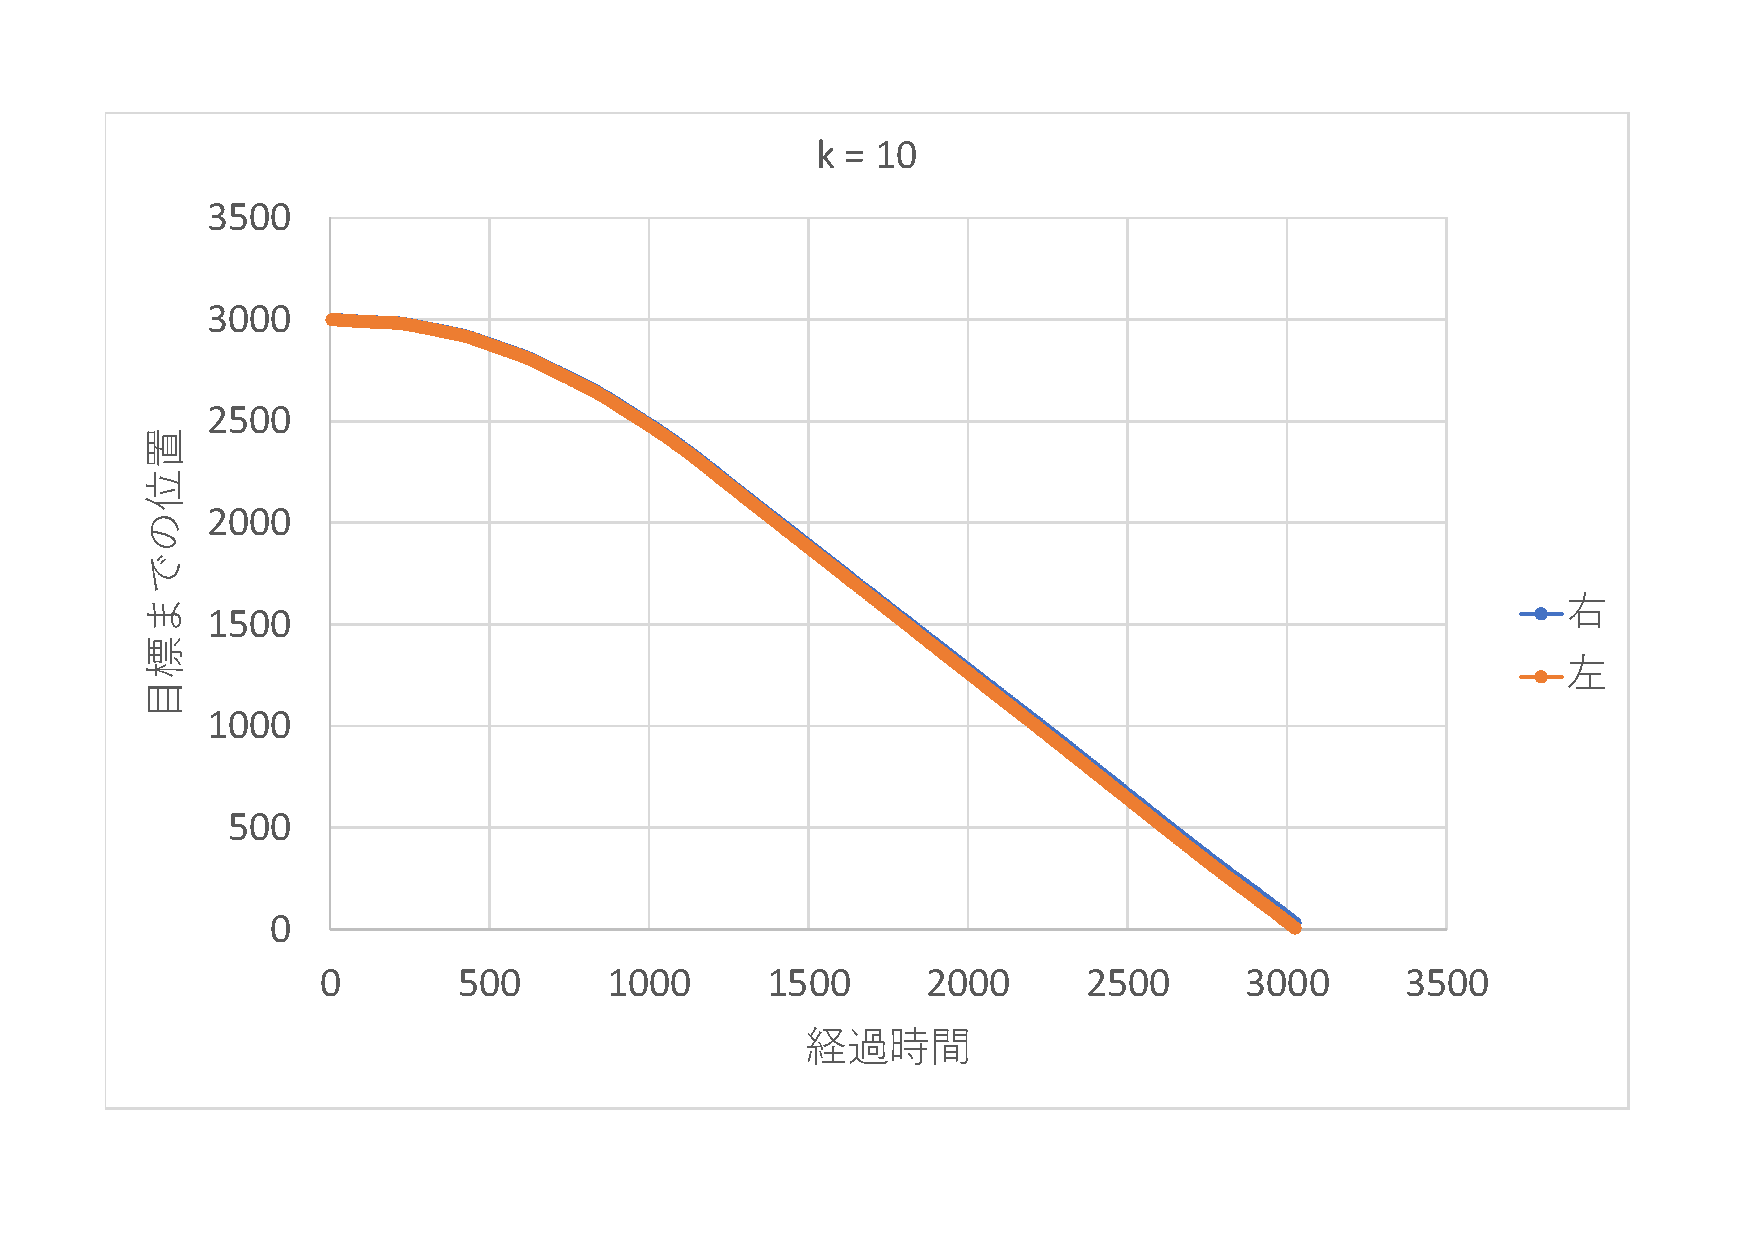
\includegraphics[width=\linewidth]{img/17/17_non_K10.pdf}
  \label{im41}
  }
  \caption{$k=10$のステップ応答}
  \end{center}
\end{figure}

\mysection{演習18}
\subsection{実行プログラム}
実行プログラムをソースコード\ref{s18}に示す。

\begin{lstlisting}[caption=演習18のプログラム,label=s18]
#include <stdio.h>
#include <math.h>
#include <process.h>
#include <dos.h>
#include "v25.h"
#include "ms.h"

#define D2R         (M_PI/180)
#define R2D         (180/M_PI)
#define RADIUS	15.0
#define DISTANCE    34.0
#define REDUCTION   19.225
#define CPR         400
#define MMPS        (60*REDUCTION/(2.0*M_PI*RADIUS))
#define DPC         (2.0*M_PI*RADIUS/((float)CPR*REDUCTION))
#define APC         (DPC/(2*DISTANCE))
#define DMAX        1000
#define THRESH_D    10
#define THRESH_Q    5*D2R
#define THRESH_V    50

#define ABS(x)      (x<0?-(x):(x))

void estimate(double *px,double *py,double *pq,long *pt);
void translate(double d,double vmax,double gain);
void rotate(double qd,double wmax,double gain);

int k=0;
int xi[DMAX],yi[DMAX],qi[DMAX];
long ti[DMAX];

int main(void)
{
    double x,y,q;
    int i;
    int kp=8,ki_inv=8;
    int vmax = 100;
    int wmax = 100/DISTANCE;
    int nl,nr;
    long t,nt;
    FILE *fp;

    ms_init();
    ms_motor_on();
    ms_set_gain(kp,ki_inv);

    estimate(&x,&y,&q,&t);
    rotate(360*D2R,wmax,5);
    translate(1000,vmax,5);

    ms_set_v(0,0);
    do{
        estimate(&x,&y,&q,&t);
        ms_read_v(&nl,&nr,&nt);
    }while(nl != 0 || nr != 0);

    ms_motor_off();

    if((fp=fopen("data.dat","wt"))==NULL)
    {
        printf("Can't open file...\n");
    }

    for(i=0;i<k;i++)
    {
        fprintf(fp,"%5d %5d %5d %5ld\n",xi[i],yi[i],qi[i],ti[i]);
    }
    fclose(fp);
    return 0;
}

void estimate(double *px,double *py,double *pq,long *pt)
{
    static long cl0=0,cr0=0;
    static double x=0.0,y=0.0,q=0.0;
    long cl,cr,ct;
    int dl,dr;
    double ds;

    ms_read_c(&cl,&cr,&ct);
    dl=cl-cl0;
    dr=cr-cr0;
    cl0=cl;
    cr0=cr;
    ds=DPC/2*(dr+dl);
    x += ds*cos(q);
    y += ds*sin(q);
    q += APC*(dr-dl);

    *px=x;
    *py=y;
    *pq=q;
    *pt=ct;
    if (k<DMAX)
    {
        xi[k]=10*x;
        yi[k]=10*y;
        qi[k]=1000*q;
        ti[k]=ct;
        k++;
    }    

}

void translate(double d,double vmax,double gain)
{
    double x0,y0,q0,x,y,q;
    long t0,t,nt;
    double cosq0,sinq0,dd,vc;
    int nc,nl,nr;

    estimate(&x0,&y0,&q0,&t0);
    cosq0=cos(q0);
    sinq0=sin(q0);
    x=x0;
    y=y0;
    q=q0;
    t=t0;

    do
    {
        dd=cosq0*(x-x0)+sinq0*(y-y0);
        vc=gain*(d-dd);
        if (ABS(vc)>vmax)
        {
            vc=(vc<0.0)?-vmax:vmax;
        }
        nc=vc*MMPS;
        ms_set_v(nc,nc);
        estimate(&x,&y,&q,&t);
        ms_read_v(&nl,&nr,&nt);
    } while (ABS(d-dd)>THRESH_D||ABS(nl)>THRESH_V||ABS(nr)>THRESH_V);
}

void rotate(double qd,double wmax,double gain)
{
  double x0,y0,q0,x,y,q;
  long t0,t,nt;
  double qq,wc,v,dw;
  int nl,nr;

  estimate(&x0,&y0,&q0,&t0);
  x=x0;
  y=y0;
  q=q0;
  t=t0;

  do{
  qq=q-q0;
  wc=gain*(qd-qq);
  if(ABS(wc)>wmax)
  {
    wc=(wc<0.0) ? -wmax:wmax;
  }
  dw=DISTANCE*wc;
  nl=-MMPS*dw;
  nr=MMPS*dw;
  ms_set_v(nl,nr);
  estimate(&x,&y,&q,&t);
  ms_read_v(&nl,&nr,&nt);
  }while (ABS(qd-qq)>THRESH_Q||ABS(nl)>THRESH_V||ABS(nr)>THRESH_V);
}
\end{lstlisting}

\mysubsection{実行結果}
ロボットが、その場で360度回転して1000[mm]直進する。
回転角度が360度ちょうどであるが、直進動作時に、
左右のモータの始動に差が生じるため、始動の遅いモータの方に
やや曲がってから直進する現象が生じた。